% !TEX program = pdflatex
% !TEX options = -synctex=1 -interaction=nonstopmode -file-line-error --shell-escape
\documentclass[sigconf,nonacm,screen,review,balance=false]{acmart}

\AtBeginDocument{%
  \providecommand\BibTeX{{%
    Bib\TeX}}}

\setcopyright{cc}
\setcctype{by-sa}
\copyrightyear{2023}

%!TEX root = ./paper.tex
\usepackage{cleveref}
\usepackage{subcaption}
\usepackage{adjustbox}
\usepackage{graphicx}
\usepackage{xcolor}

\definecolor {codeBackground} {HTML} {F4F4F4} % {F7F7F7} AYU common.bg
\definecolor {codeForeground} {HTML} {000000} % AYU common.fg
\definecolor {codeKeyword}    {HTML} {399EE6} % AYU syntax.entity
\definecolor {codeBuiltin}    {HTML} {55B4D4} % AYU syntax.tag
\definecolor {codeConstant}   {HTML} {A37ACC} % AYU syntax.constant
\definecolor {codeString}     {HTML} {86B300} % AYU syntax.string
\definecolor {codeEmph}       {HTML} {FA8D3E} % AYU syntax.keyword
\definecolor {codeRuler}      {HTML} {CACACA} % AYU ui.panel.border
\definecolor {codeComment}    {HTML} {8A9199} % AYU common.ui
\definecolor {codeIdentifier} {HTML} {1c1c1c}
\definecolor {codeOperator}   {HTML} {4CBF99}
\definecolor {codeError}      {HTML} {E65050} % AYU common.error

\usepackage[flushleft,alwaysadjust]{paralist}
\AtBeginDocument{\setdefaultleftmargin{0.7em}{}{}{}{}{}}

\crefname{option}{option}{options}
\Crefname{option}{Option}{Options}

\usepackage{relsize}
\usepackage{twemojis}
\usepackage{fancyvrb}
\usepackage{listings}
\lstset{
  inputencoding=utf8,
  basicstyle=\ttfamily\mdseries,
  fancyvrb=true,
  sensitive=true,
  numberstyle=\smaller[2]\ttfamily\color{codeRuler},
  numberblanklines=false,
  %breaklines=true,
  extendedchars=false, showstringspaces=false, columns=fixed, stepnumber=1,
  escapeinside={\%*}{*)}, lineskip=-5pt, basewidth=0.5em }

\definecolor{pc}{HTML}{55B4D4}
\definecolor{branching}{HTML}{FA8D3E}
\definecolor{arithmetic}{HTML}{ED9366}
\definecolor{stack}{HTML}{A37ACC}
\definecolor{userio}{HTML}{4CBF99}
\definecolor{gridio}{HTML}{86B300}
\definecolor{stringmode}{HTML}{FF7383}
\definecolor{endprogram}{HTML}{E65050}
\definecolor{ignore}{HTML}{787B80}
\definecolor{number}{HTML}{5C6166}
\definecolor{codebg}{HTML}{F3F4F5}

\colorlet{stringbg}{stringmode!20}
\colorlet{pcbg}{pc!20}
\colorlet{branchingbg}{branching!20}

\newcommand{\keyword}[1]{{\color{codeKeyword}\bfseries\ttfamily #1}}

\lstdefinelanguage{sql}{
basicstyle=\linespread{1.0}\color{codeForeground}\ttfamily\mdseries,
identifierstyle=\color{codeIdentifier},
commentstyle=\color{codeComment},
stringstyle=\color{codeString},
emphstyle={\color{codeEmph}\itshape\bfseries},
keywordstyle={[1]\color{codeKeyword}\bfseries},
keywordstyle={[2]\color{codeBuiltin}\bfseries},
keywordstyle={[3]\color{codeConstant}\bfseries},
keywordstyle={[4]\color{codeOperator}\bfseries},
emptylines=*10,
morestring=[d]{'},
morecomment=[l]{--},
morekeywords=[1]{WITH,RECURSIVE,UNION,ALL,SELECT,FROM,WHERE,CASE,WHEN,THEN,END,LATERAL,AS,ITERATE,LEFT,RIGHT,OUTER,INNER,JOIN,IF,ELSE,ELSIF},
morekeywords=[2]{int4,float8,text,boolean,ARRAY,CARDINALITY,ABS,FLOOR,CEIL,ROUND,RANDOM,SIGN,MAX,MIN,ARRAY_AGG,unnest,json_each},
morekeywords=[3]{NULL,TRUE,FALSE},
morekeywords=[4]{AND,OR,NOT,BETWEEN,IS},
literate=%
{(}{{{\color{codeOperator}(}}}1
    {)}{{{\color{codeOperator})}}}1
{[}{{{\color{codeOperator}[}}}1
{]}{{{\color{codeOperator}]}}}1
% {\{}{{{\color{codeOperator}\{}}1
% {\}}{{{\color{codeOperator}\}}}1
{:}{{{\color{codeOperator}:}}}1
{.}{{{\color{codeOperator}.}}}1
{,}{{{\color{codeOperator},}}}1
{+}{{{\color{codeOperator}+}}}1
{-}{{{\color{codeOperator}-}}}1
{*}{{{\color{codeOperator}*}}}1
{/}{{{\color{codeOperator}/}}}1
{\%}{{{\color{codeOperator}\%{}}}}1
{@}{{{\color{codeOperator}@}}}1
{^}{{{\color{codeOperator}\^{}}}}1
{|}{{{\color{codeOperator}|}}}1
{\&}{{{\color{codeOperator}\&}}}1
{<}{{{\color{codeOperator}<}}}1
{>}{{{\color{codeOperator}>}}}1
{=}{{{\color{codeOperator}=}}}1
{!}{{{\color{codeOperator}!}}}1
{...}{{{\color{codeComment}...}}}3
}
\newcommand{\sql}[1]{\text{\lstinline[language=sql]!#1!}}

\lstdefinelanguage{py}{
basicstyle=\linespread{1.0}\color{codeForeground}\ttfamily,
identifierstyle=\color{codeIdentifier},
commentstyle=\color{codeComment},
stringstyle=\color{codeString},
emphstyle={\color{codeEmph}\itshape\bfseries},
keywordstyle={[1]\color{codeKeyword}\bfseries},
keywordstyle={[2]\color{codeBuiltin}\bfseries},
keywordstyle={[3]\color{codeConstant}\bfseries},
keywordstyle={[4]\color{codeOperator}\bfseries},
emptylines=*10,
morestring=[d]{"},
morecomment=[l]{\#},
morekeywords=[1]{def,for,while,if,else,try,except,finally,yield,async,await,return,match,case,switch,do},
morekeywords=[2]{int,float,bool,str,list,dict,set},
morekeywords=[3]{None,True,False},
morekeywords=[4]{is,not,in,and,or},
literate=%
{(}{{{\color{codeOperator}(}}}1
    {)}{{{\color{codeOperator})}}}1
{[}{{{\color{codeOperator}[}}}1
{]}{{{\color{codeOperator}]}}}1
% {\{}{{{\color{codeOperator}\{}}1
% {\}}{{{\color{codeOperator}\}}}1
{:}{{{\color{codeOperator}:}}}1
{.}{{{\color{codeOperator}.}}}1
{,}{{{\color{codeOperator},}}}1
{+}{{{\color{codeOperator}+}}}1
{-}{{{\color{codeOperator}-}}}1
{*}{{{\color{codeOperator}*}}}1
{/}{{{\color{codeOperator}/}}}1
{\%}{{{\color{codeOperator}\%{}}}}1
{@}{{{\color{codeOperator}@}}}1
{^}{{{\color{codeOperator}\^{}}}}1
{|}{{{\color{codeOperator}|}}}1
{\&}{{{\color{codeOperator}\&}}}1
{<}{{{\color{codeOperator}<}}}1
{>}{{{\color{codeOperator}>}}}1
{==}{{{\color{codeOperator}==}}}2
{!=}{{{\color{codeOperator}!=}}}2
{<=}{{{\color{codeOperator}<=}}}2
{>=}{{{\color{codeOperator}>=}}}2
{...}{{{\color{codeComment}...}}}3
{=}{{{\color{codeConstant}=}}}1
}
\newcommand{\py}[1]{\text{\lstinline[language=py]!#1!}}

\lstdefinelanguage{befunge}{
basicstyle=\ttfamily\mdseries\color{ignore},
literate=%
{^}{{{\color{pc}\^{}}}}1
{<}{{{\color{pc}<}}}1
{>}{{{\color{pc}>}}}1
{v}{{{\color{pc}v}}}1
{?}{{{\color{pc}?}}}1
{\#}{{{\color{pc}\#}}}1
{|}{{{\color{branching}|}}}1
{\_}{{{\color{branching}\_}}}1
{+}{{{\color{arithmetic}+}}}1
{-}{{{\color{arithmetic}-}}}1
{*}{{{\color{arithmetic}*}}}1
{/}{{{\color{arithmetic}/}}}1
{\%}{{{\color{arithmetic}\%{}}}}1
{\!}{{{\color{arithmetic}!}}}1
{\`}{{{\color{arithmetic}\`{}}}}1
{:}{{{\color{stack}:}}}1
{\\}{{{\color{stack}\textbackslash}}}1
{\$}{{{\color{stack}\$}}}1
{.}{{{\color{userio}.}}}1
{,}{{{\color{userio},}}}1
{&}{{{\color{userio}\&}}}1
{~}{{{\color{userio}\~{}}}}1
{g}{{{\color{gridio}g}}}1
{p}{{{\color{gridio}p}}}1
{"}{{{\color{stringmode}"}}}1
{@}{{{\color{endprogram}@}}}1
{0}{{{\color{number}0}}}1
{1}{{{\color{number}1}}}1
{2}{{{\color{number}2}}}1
{3}{{{\color{number}3}}}1
{4}{{{\color{number}4}}}1
{5}{{{\color{number}5}}}1
{6}{{{\color{number}6}}}1
{7}{{{\color{number}7}}}1
{8}{{{\color{number}8}}}1
{9}{{{\color{number}9}}}1
}
\newcommand{\befunge}[1]{\text{\lstinline[basicstyle=\ttfamily\mdseries\small,language=befunge]!#1!}}
\newcommand{\stringStyle}[1]{{\lstinline[basicstyle=\ttfamily\mdseries\color{stringmode}]!#1!}}

% \lstdefinelanguage{intercal}{
%   basicstyle=\ttfamily\mdseries\color{ignore}
% }
% \newcommand{\please}[1]{\text{\lstinline[basicstyle=\ttfamily\mdseries\small,language=intercal]!#1!}}

\lstdefinelanguage{brainfuck}{
basicstyle=\ttfamily\mdseries\color{ignore},
literate=%
  {<}{{{\color{pc}<}}}1
{>}{{{\color{pc}>}}}1
{[}{{{\color{branching}[}}}1
{]}{{{\color{branching}]}}}1
{+}{{{\color{arithmetic}+}}}1
{-}{{{\color{arithmetic}-}}}1
{.}{{{\color{userio}.}}}1
{,}{{{\color{userio},}}}1
}
\newcommand{\brainfuck}[1]{\text{\lstinline[language=brainfuck]!#1!}}

\usepackage{adjustbox}

%% TikZ ist kein Zeichenprogramm
\usepackage{tikz}
\usetikzlibrary{arrows.meta}
\usetikzlibrary{bending}
\usetikzlibrary{patterns}
\usetikzlibrary{shapes.symbols}
\usetikzlibrary{shapes.multipart}
\usetikzlibrary{shapes.misc}
\usetikzlibrary{shadows}
\usetikzlibrary{shadings}
\usetikzlibrary{calc}
\usetikzlibrary{fit}
\usetikzlibrary{decorations.pathreplacing}
%% layered TiKZ drawings
\pgfdeclarelayer{background}
\pgfdeclarelayer{foreground}
\pgfsetlayers{background,main,foreground}
%% TikZ-based (scatter) plots
\usepackage{pgfplots}
%% read table cells from CSV input
\usepackage{pgfplotstable}
\usepackage{pgffor}
\usetikzlibrary{fpu}
%% make sure that TikZ's calc library and lstlisting's 'mathescape=true' cooperate
\makeatletter
\global\let\tikz@ensure@dollar@catcode=\relax
\makeatother

%% lengths that measure character box width and height in code/in a listing
\newlength{\x}
\newlength{\y}
\newlength{\xx}

\colorlet{linear}{codeEmph}
\colorlet{nonlinear}{codeConstant}
\colorlet{branching}{codeString}

\newcommand{\linearCFarrow}{
  \begin{tikzpicture}[x=1.75ex,y=1.75ex,inner sep=0pt,outer sep=0pt]
    \draw[-{Latex[round,length=1.0ex,width=0.6ex]},line cap=round,line width=0.175ex] (0,1) -- (0,0);
  \end{tikzpicture}}

\newcommand{\linearCF}{
  
\begin{tikzpicture}[x=2ex,y=3ex,inner sep=0pt,outer sep=0pt,baseline={([yshift=-.75ex]current bounding box.center)}]
    \fill[linear,rounded corners=2pt] (0,0) rectangle (1,1);
    \node[linear!25] at (0.5,0.45) {\linearCFarrow};
  \end{tikzpicture}}

\newcommand{\branchingCFarrow}{
  
\begin{tikzpicture}[x=1.75ex,y=1.75ex,inner sep=0pt,outer sep=0pt]
    \coordinate (split) at (0,0.7);
    \begin{scope}[line width=0.175ex,rounded corners=0.3ex,line cap=round]
      \draw                                            (0,1.0) -- (split);
      \draw[-{Latex[round,length=1.0ex,width=0.6ex]}] (split) -- +(-0.2,0) -- (-0.2,0);
      \draw[-{Latex[round,length=1.0ex,width=0.6ex]}] (split) -- +( 0.2,0) -- ( 0.2,0);
    \end{scope}
  \end{tikzpicture}}

\newcommand{\branchingCF}{
  
\begin{tikzpicture}[x=2ex,y=3ex,inner sep=0pt,outer sep=0pt,baseline={([yshift=-.75ex]current bounding box.center)}]
    \fill[branching,rounded corners=2pt] (0,0) rectangle (1,1);
    \node[branching!25] at (0.5,0.45) {\branchingCFarrow};
  \end{tikzpicture}}

\newcommand{\nonlinearCFarrow}{
  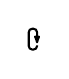
\begin{tikzpicture}[x=1.75ex,y=1.75ex,inner sep=0pt,outer sep=0pt]
    \coordinate (split) at (0,0.7);
    \begin{scope}[line width=0.175ex,rounded corners=0.3ex]
      \draw[-{Latex[round,length=1.0ex,width=0.6ex]}] (0.2,0.2) -- (0.2,0.0) -- (-0.2,0.0) -- (-0.2,1.0) -- (0.2,1.0) -- (0.2,0.3);
    \end{scope}
  \end{tikzpicture}}

\newcommand{\nonlinearCF}{
  
\begin{tikzpicture}[x=2ex,y=3ex,inner sep=0pt,outer sep=0pt,baseline={([yshift=-.75ex]current bounding box.center)}]
    \fill[nonlinear,rounded corners=2pt] (0,0) rectangle (1,1);
    \node[nonlinear!25] at (0.55,0.5) {\nonlinearCFarrow};
  \end{tikzpicture}}

\newsavebox{\linearCFbox}\savebox{\linearCFbox}{\linearCF}
\newsavebox{\nonlinearCFbox}\savebox{\nonlinearCFbox}{\nonlinearCF}
\newsavebox{\branchingCFbox}\savebox{\branchingCFbox}{\branchingCF}

\newcommand{\circled}[1]{
  \begin{tikzpicture}[outer sep=0pt,inner sep=0pt,baseline={(circ.base)}]
    \node[circle,draw=.,fill=.!25,inner sep=0.2ex,line width=0.2ex,anchor=base] (circ) {#1};
  \end{tikzpicture}
}

\newcommand{\cfoption}[2]{\hspace{-0.4em}\mbox{\bfseries\ttfamily\color{#1}\smaller\circled{#2}}\hspace{-0.4em}}


\begin{document}

\title{Befunge-93 in SQL}
\subtitle{(Ab-)Using SQL's Turing Completeness}

\author{Tim Fischer}
\email{t.fischer@student.uni-tuebingen.de}
\orcid{0000-0002-6625-9627}
\affiliation{%
  \institution{Eberhard Karls Universität}
  \streetaddress{Sand 13}
  \city{Tübingen}
  \state{Baden-Württemberg}
  \country{Germany}
  \postcode{72076}
}

\begin{abstract}
  Though SQL has been Turing complete since the SQL:1999 standard leveraging
  this feature to full effect still eludes many developers. One of the major
  roadblocks standing the way is the conceptual impedance mismatch between SQL's
  declarative semantics and the imperative semantics most developers are more
  familiar with. Where this becomes most evident is when trying to express
  complex control flow such as chained assignments, loops, and branches in a
  generic manner. In this seminar paper, we introduce techniques to represent
  such control flow constructs in plain SQL:1999 and demonstrate their use by
  implementing an interpreter for the esoteric programming language Befunge.
\end{abstract}

\keywords{SQL, Befunge, Interpreters, Recursion}

\maketitle

\section{Introduction}

To the layman, programming languages appear to be magical incantations that
allow ``computer wizards'' to make computers obey their every whim. This
mysticism around programming languages does not leave novice disciples of
programming; the first fact they learn is that when developing these supposed
magical incantations in any given programming language, they need to adhere to
a strict set of rules. Comprising these rules are two major parts:
\emph{syntax} and \emph{semantics}.

Though at first both \emph{syntax} and \emph{semantics} appear arbitrary at
best, deeper study reveals the logic behind them. More often than not
programming languages are built around a small set of core features that
dictate the design of their semantics and syntax. For example, LISP
\cite{mccarthy1962lisp} is built, both semantically and syntactically, around
the concept of list-based symbolic processing.

Not all language design concepts are equally as expressive in all domains. Take
Smalltalk \cite{kay1993smalltalk}, for example, it is a language in which all
code is structured around the concept of objects that interact with one
another. SQL \cite{chamberlin2012historysql} on the other hand is a query
language the main goal of which is to enable developers to query relational
data in a declarative manner.

When evaluating the expressiveness of programming language design concepts the
property of Turing completeness elevates some languages above others. Though
not a necessary property, for a language to be actually ``useful'', it
nonetheless allows for gauging what kinds of programs can be expressed. In
short, a Turing complete language can express any problem a Turing machine can
solve and is thus capable of expressing most ``sensible'' computations.

All the programming languages referenced so far are Turing complete, this
includes the obvious two, LISP and Smalltalk, and also, maybe surprisingly so,
SQL. SQL has been Turing complete since the introduction of recursive common
table expressions (\keyword{WITH RECURSIVE}) in the 1999 standard \cite
{sql-1999}. Which allow SQL developers to express any Turing complete problem
in terms of fixpoint computation.

SQL's Turing completeness, in theory, allows developers to make use of textbook
algorithms like the Dijkstra algorithm or the Edmonds-Karp algorithm; both of
which are algorithms that can be used in many situations. In practice, however,
developers opt to side-step writing these algorithms in SQL in favor of
imperative languages. This often comes down to the impedance mismatch between
the imperative pseudocode most textbooks depict these algorithms in and the
declarative nature of SQL code.

In this paper, we will flex SQL's Turing complete muscles by demonstrating how to
translate a Python-based Befunge interpreter into a single recursive SQL:1999
query in three major steps.
\begin{itemize}
  \item In \Cref{sec:eso-langs}, we will look at what constitutes esoteric
        programming languages and what Befunge is. In doing so we will also
        argue why Befunge is an interesting vehicle for our cause.
  \item In \Cref{sec:py-inter}, we will deconstruct an imperative Befunge
        interpreter into a general program shape and the individual types of
        control flow residing within.
  \item In \Cref{sec:flexing}, we will translate the Python-based Befunge
        interpreter into a recursive query; all the while only making
        use SQL:1999.
\end{itemize}

\begin{figure*}
  \begin{adjustbox}{center}
    \begin{subfigure}{0.275\textwidth}
      \centering
      %% measure the width of xx in a listing
      \settowidth{\xx}{\lstinline[columns=fixed]{xx}}\setlength{\x}{0.5\xx}
      \setlength{\y}{2ex}
      \begin{tikzpicture}[x=\x,y=-\y,inner sep=0mm]
        \node[anchor=north west] at (0,0) {%
          \begin{lstlisting}[language=befunge,gobble=12]
            "!dlroW ,olleH">:#v_@
                            ^ ,<
          \end{lstlisting}%
        };
        \begin{pgfonlayer}{background}
          \fill[codebg,rounded corners=1pt] (-1,-0.5) rectangle (22,2.5);
        \end{pgfonlayer}
      \end{tikzpicture}
      \caption{Hello World}
      \label{fig:example-hello-world}
    \end{subfigure}
    \hfill
    \begin{subfigure}{0.175\textwidth}
      \centering
      %% measure the width of xx in a listing
      \settowidth{\xx}{\lstinline[columns=fixed]{xx}}\setlength{\x}{0.5\xx}
      \setlength{\y}{2ex}
      \begin{tikzpicture}[x=\x,y=-\y,inner sep=0mm]
        \node[anchor=north west] at (0,0) {%
          \begin{lstlisting}[language=befunge,gobble=12]
            &>:1-:v v *_$.@
              ^    _$>\:^
          \end{lstlisting}%
        };
        \begin{pgfonlayer}{background}
          \fill[codebg,rounded corners=1pt] (-1,-0.5) rectangle (16,2.7);
        \end{pgfonlayer}
      \end{tikzpicture}
      \caption{Factorial}
      \label{fig:example-factorial}
    \end{subfigure}
    \hfill
    \begin{subfigure}{0.55\textwidth}
      \centering
      %% measure the width of xx in a listing
      \settowidth{\xx}{\lstinline[columns=fixed]{xx}}\setlength{\x}{0.5\xx}
      \setlength{\y}{2ex}
      \begin{tikzpicture}[x=\x,y=-\y,inner sep=0mm]
        \node[anchor=north west] at (0,0) {%
          \begin{lstlisting}[language=befunge,gobble=12]
            211p&01p>121p          >21g1+21p 11g21g-v>11g21g%#v_v
                                                    >|
                             v,,,,, ,,,.g11"is prime"<
            >       ^        >   v ^                          <
            ^_@#-g10p11:+1g11,*25<,,,,,,,,,,,,.g11"is not prime"<
          \end{lstlisting}%
        };

        \begin{pgfonlayer}{background}
          \fill[codebg,rounded corners=1pt] (-1,-0.5) rectangle (54,6);
        \end{pgfonlayer}
      \end{tikzpicture}
      \caption{Prime Numbers}
      \label{fig:example-prime}
    \end{subfigure}
  \end{adjustbox}
  \caption{A collection of sample programs written in Befunge in increasing complexity.}
  \label{fig:examples}
\end{figure*}

\section{Esoteric Programming Languages}
\label{sec:eso-langs}

Amongst all the groups of programming languages in which language designers like
to claim their creations are Turing complete, one foregoes the most basic of
constraints of making both the language's semantics and syntax sensible to
read, write, let alone, reason in and about. Programming languages in this
group are known as \emph{esoteric programming languages}\cite
{fuller2008software,mateas2005darkly}.

One of the earliest examples of such a programming language is INTERCAL which
was written by Don Wood and James Lyon in 1972 and revived by Eric S. Raymond
in 1990 \cite{intercal}. INTERCAL's sole design tenet is to satirize as many
aspects of other programming languages as possible. For example, a proper
INTERCAL program must contain an entirely undefined amount of the
\keyword{PLEASE} keyword; too few and the compiler rejects the input program
 for \emph{impoliteness}, too many and the compiler rejects for \emph
 {excessive politeness}.

Some esoteric programming languages take a more minimal approach, the most
well-known examples of this are Wouter van Oortmerssen's FALSE \cite{false} and
Urban Müller's Brainfuck \cite{brainfuck}. A simple \emph
{cat program}\footnotemark in the latter can be written as
\brainfuck{,+[-.,+]}. Both make use of a minimal amount of syntactic and
 semantic constructs to express arbitrarily complex computations. In short,
 Brainfuck simulates a Turing machine in a very direct manner, and FALSE
 operates what is known as a stack machine.

\footnotetext{A \emph{cat program} is a program that simply copies its standard
input to its standard output.}

Brainfuck especially has become synonymous with esoteric programming languages
in general. Aside from both its simplicity and absurdity, a core reason is
that it is a Turing complete language \cite{bfTuringComplete} that is fairly
direct to be understood as such. This feature has made Brainfuck the go-to
target for reduction arguments concerning Turing completeness. Any language
which can be used to implement a Brainfuck interpreter, with an ``infinite''
number of memory cells\footnotemark, is, in fact, Turing complete.

\footnotetext{In reality this is mostly a soft requirement for the most part, as
 many languages limit the program/stack/heap/etc. size artificially. The
 original Brainfuck reference implementation limited the number of memory cells
 to 30000.}

\subsection{Befunge}
\label{sec:befunge}

Another esoteric programming language that follows in the footsteps of the likes
of FALSE and Brainfuck is Befunge-93 \cite{befunge} (from here on just
Befunge). Befunge was invented by Chris Pressey in 1993 with the express intent
to be difficult to compile. Befunge is a Turing complete, stack-based,
self-modifying, two-dimensional language.

Befunge programs are arranged on a 2D character grid, dubbed the funge space,
and each character represents a single command. At runtime, this funge space is
traversed by the program counter, which can be in one of two execution modes:
normal mode and string mode. During operation in normal mode, each command
character the program counter ``lands on'' is executed, and any non-command
character is treated as a comment. Some commands change the travel direction or
step length of the program counter, some interact with the program stack to
perform basic calculations and the like. In string mode, which is toggled by
the \befunge{"} character, the ASCII value of all encountered characters is
pushed onto the stack until the execution mode is toggled back.

In 1998, Pressey sought to extend both the feature set and the number of
dimensions available in Befunge programs. In this process, he created then
Funge-98 family of languages \cite{befunge98}. Aside from the newly introduced
commands it also lifts the program size restriction of Befunge-93, which was
capped at 80$\times$25 characters. Without this size constraint, it is commonly
accepted that Befunge-93 is Turing-complete, and with just a few Funge-98
specific commands it is possible to implement a Brainfuck interpreter
\cite{bfInBefunge}.

In this paper, we are working towards showing the expressibility of
Turing-complete control flow in SQL in a direct but fun manner. And as any
Turing-complete language can be used to implement an interpreter for any other
Turing-complete language, this makes a Befunge\footnotemark{} interpreter a
suitable sample program to flex SQL's muscles.

\footnotetext{The actual version of Befunge we are targeting is Befunge-93
 without the program size constraint.}

\section{Imperative Befunge Interpreter}
\label{sec:py-inter}

There are many ways to styles of interpreters---tree-walk interpreters, bytecode
interpreters, graph reduction interpreters, etc. Befunge lends itself to
VM-like interpreters. Such interpreters are similar in style to bytecode
interpreters, in that they emulate very simple semantics, the difference stems
from VM-style interpreters not needing to compile given programs into bytecode
beforehand. In short, our interpreter will retain the running program in
exactly the form Befunge programs are supplied, in a 2D grid of ASCII values.

\begin{figure}[t]
  \centering
  %% measure the width of xx in a listing
  \settowidth{\xx}{\lstinline[columns=fixed]{xx}}\setlength{\x}{0.5\xx}
  \setlength{\y}{2ex}
  \begin{tikzpicture}[x=\x,y=-\y,inner sep=0mm]
    \node[anchor=north west] at (0,0) {%
      \begin{lstlisting}[language=py,gobble=8,numbers=left,label={lst:python-inter-skeleton}]
        def interpreter(source):
            program = preprocess(source)
            state   = make_inital_state(program)

            while state.mode != "%*\texttwemoji{chequered flag}*)":

                match state.mode:
                    case "%*\texttwemoji{gear}*)": ...
                    case "%*\texttwemoji{sewing needle}*)": ...

                match state.direction:
                    case "%*\texttwemoji{right arrow}*)": ...
                    case "%*\texttwemoji{down arrow}*)": ...
                    case "%*\texttwemoji{left arrow}*)": ...
                    case "%*\texttwemoji{up arrow}*)": ...


          return state.result
      \end{lstlisting}%
    };
    \begin{pgfonlayer}{background}
      \begin{scope}[rounded corners=2pt]
        \fill[codebg]                                          (-1.50,-0.50) rectangle (42.25,20.00);

        \fill[linear,draw=linear,line width=1.7pt]         ( 2.25, 1.25) rectangle (40.75, 3.45);
        \fill[linear!25]                                     ( 3.65, 1.25) rectangle (40.75, 3.45);

        \fill[nonlinear,draw=nonlinear,line width=1.7pt] ( 2.25, 4.35) rectangle (40.75,17.50);
        \fill[nonlinear!25]                                 ( 3.65, 4.35) rectangle (40.75,17.50);

        \fill[linear,draw=linear,line width=1.7pt]         ( 4.25, 5.85) rectangle (39.75,17.00);
        \fill[linear!25]                                     ( 5.65, 5.85) rectangle (39.75,17.00);

        \fill[branching,draw=branching,line width=1.7pt]     ( 6.25, 6.35) rectangle (38.75, 9.95);
        \fill[branching!25]                                   ( 7.65, 6.35) rectangle (38.75, 9.95);

        \fill[branching,draw=branching,line width=1.7pt]     ( 6.25,10.65) rectangle (38.75,16.50);
        \fill[branching!25]                                   ( 7.65,10.65) rectangle (38.75,16.50);
      \end{scope}
      \begin{scope}[inner sep=0pt,outer sep=0pt,every node/.style={anchor=center}]
        \node[linear!25]     at (2.90, 2.00) {\linearCFarrow};
        \node[nonlinear!25] at (2.95, 5.05) {\nonlinearCFarrow};
        \node[linear!25]     at (4.90, 6.60) {\linearCFarrow};
        \node[branching!25]   at (6.85, 7.05) {\branchingCFarrow};
        \node[branching!25]   at (6.85,11.35) {\branchingCFarrow};
      \end{scope}
    \end{pgfonlayer}
  \end{tikzpicture}
  \caption{Python-based skeleton implementation of a Befunge interpreter written
   in an iterative style and highlighted control flow regions.}
  \label{fig:python-inter-skeleton}
\end{figure}

\Cref{fig:python-inter-skeleton} shows a rough sketch of a Befunge interpreter
 written in Python. Though not complete, the missing parts---i.e., the \py
 {...}-parts---are just more branching, some array-based stack manipulation,
 and simple integer arithmetic. The translation methods we will discuss extend
 naturally over those parts as well. Both the complete translation and some
 Python scripts to make the SQL-based interpreter more useable can be found on
 Codeberg\footnotemark{}.

\footnotetext{The Git-Repository can be found at \url
 {https://codeberg.org/timfi/befunge-sql}.}

The interpreter ingests Befunge source code as a string which is first
transformed into a 2D array for easier access. Afterward, we prepare the
interpreter state which contains the funge space, the program counter, the
stack and the execution mode. This program state is then iterated over until
the execution mode signals termination. This iteration follows in two steps;
in the first step, the interpreter ingests and processes the character the
program counter resides on per the current processing mode. In the second
step, the interpreter moves the program counter to the next character based on
either the preexisting movement direction and step width or possibly updated
variants of the two. On program termination, the interpreter then returns the
generated output.

\subsection{Concessions to Codd}

In preparation for translating the interpreter to SQL, we need to make some
concessions. Though Turing complete, there are some features that SQL does not
and most likely will never support as they are entirely out of scope for a
database query language. The biggest necessary concession is interactive I/O;
Befunge's input and output commands usually interact directly with standard
input and standard output, both of which SQL cannot interact with. To meet
halfway our interpreter takes input up-front and returns all output at once
upon completion.

% [TODO] funge space size

\subsection{Types of Control Flow}
\label{sec:cf-types}

\begin{figure}[t]
  \centering
  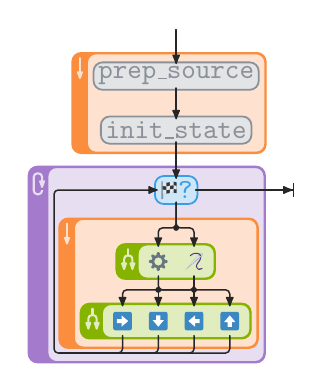
\begin{tikzpicture}[x=1ex,y=-2ex,inner sep=0pt]
    %% query parts
    \begin{scope}[every node/.style={font=\ttfamily\mdseries,minimum height=1.5ex,anchor=base}]
      \node[codeComment] at ( 0.0,-0.5) (prep)    {prep\_source};
      \node[codeComment] at ( 0.0, 2.0) (state)   {init\_state};
      \node[codeKeyword] at ( 0.0, 4.5) (check)   {\texttwemoji{chequered flag}?};
      \node[codeString]  at (-1.5, 7.5) (process) {\texttwemoji{gear}};
      \node[codeString]  at ( 1.5, 7.5) (string)  {\texttwemoji{sewing needle}};
      \node[codeString]  at (-4.5,10.0) (right)   {\texttwemoji{right arrow}};
      \node[codeString]  at (-1.5,10.0) (down)    {\texttwemoji{down arrow}};
      \node[codeString]  at ( 1.5,10.0) (left)    {\texttwemoji{left arrow}};
      \node[codeString]  at ( 4.5,10.0) (up)      {\texttwemoji{up arrow}};
    \end{scope}
    \coordinate (through1) at (  0.00, 5.75);
    \coordinate (through2) at (  0.00, 8.35);
    \coordinate (through3) at (-10.25,11.00);

    %% transitions
    \begin{scope}[%
        line cap=round,%
        rounded corners=0.35ex,%
        line width=0.125ex,%
        goto/.tip={Latex[round,length=1ex]},%
        return/.tip={Latex[round,length=1ex] Bar},%
        every path/.style={shorten >=0.1ex,shorten <=0.2ex},%
        draw=black!85,%
        fill=black!85,%
      ]
      \fill[radius=0.25ex] (through1) circle node (branch1) {};
      \fill[radius=0.25ex] (process |- through2) circle node (branch2) {};
      \fill[radius=0.25ex] (string |- through2) circle node (branch3) {};

      \draw[{goto}-]   (prep)    to +(0,-2);
      \draw[-{goto}]   (prep)    to (state);
      \draw[-{goto}]   (state)   to (check);
      \draw[-{return}] (check)   to +(10,0);

      \draw[-{goto},shorten >=0.4ex]   (check)   to (through1) to (process |- through1) to (process);
      \draw[-{goto},shorten >=0.4ex]   (check)   to (through1) to (string |- through1)  to (string);

      \draw[-{goto},shorten >=0.4ex,shorten <=0.4ex] (process)                                                 to (down);
      \draw[-{goto},shorten >=0.4ex,shorten <=0.4ex] (process) to (process |- through2) to (up |- through2)    to (up);

      \draw[-{goto},shorten >=0.4ex,shorten <=0.4ex] (string)  to (string |- through2)  to (right |- through2) to (right);
      \draw[-{goto},shorten >=0.4ex,shorten <=0.4ex] (string)                                                  to (left);

      \draw[-{goto},shorten <=0.4ex]       (up)    to (up    |- through3) to (through3) to (through3 |- check) to (check);
      \draw[shorten >=2pt,shorten <=0.4ex] (left)  to (left  |- through3) to (through3);
      \draw[shorten >=2pt,shorten <=0.4ex] (down)  to (down  |- through3) to (through3);
      \draw[shorten >=2pt,shorten <=0.4ex] (right) to (right |- through3) to (through3);
    \end{scope}


    \begin{pgfonlayer}{background}
      \coordinate (loopbottom) at (through3);

      \begin{scope}[%
          rounded corners=0.75ex,%
          inner sep=0pt,%
          dummy bounding box/.style={inner xsep=0.5ex, inner ysep=0.7ex},%
          bounding box/.style={inner sep=0pt, line width=0.15ex},%
          dummy annotation/.style={anchor=center,outer sep=0.3ex},%
          annotation/.style={anchor=center},%
          dummy decoration/.style={inner sep=0.3ex},%
          decoration/.style={line width=0.15ex},%
        ]

        \node[dummy decoration, fit=(prep)   ] (_prep)    {};
        \node[dummy decoration, fit=(state)  ] (_state)   {};
        \node[dummy decoration, fit=(check)  ] (_check)   {};
        \node[dummy decoration, fit=(process)] (_process) {};
        \node[dummy decoration, fit=(string) ] (_string)  {};
        \node[dummy decoration, fit=(right)  ] (_right)   {};
        \node[dummy decoration, fit=(down)   ] (_down)    {};
        \node[dummy decoration, fit=(left)   ] (_left)    {};
        \node[dummy decoration, fit=(up)     ] (_up)      {};

        \node[dummy bounding box, fit=(_prep) (_state)] (init) {};
        \node[dummy annotation] at ($(init.north west) + (-0.6,0.7)$) (initarr) {\linearCFarrow{}};
        \node[fit=(init) (initarr)] (_init) {};

        \node[dummy bounding box,inner ysep=0.2ex, fit=(_process) (_string)] (mode) {};
        \node[dummy annotation] at ($(mode.north west) + (-0.8,0.7)$) (modearr) {\branchingCFarrow{}};
        \node[fit=(mode) (modearr)] (_mode) {};

        \node[dummy bounding box,inner ysep=0.2ex, fit=(_right) (_down) (_up) (_left)] (move) {};
        \node[dummy annotation] at ($(move.north west) + (-0.8,0.7)$) (movearr) {\branchingCFarrow{}};
        \node[fit=(move) (movearr)] (_move) {};

        \node[dummy bounding box, fit=(_move) (_mode) (through1)] (body) {};
        \node[dummy annotation] at ($(body.north west) + (-0.6,0.7)$) (bodyarr) {\linearCFarrow{}};
        \node[fit=(body) (bodyarr)] (_body) {};

        \node[dummy bounding box, fit=(_check) (_body) (loopbottom)] (loop) {};
        \node[dummy annotation] at ($(loop.north west) + (-0.7,0.7)$) (looparr) {\nonlinearCFarrow{}};
        \node[fit=(loop) (looparr)] (_loop) {};

        %% draw final bounding boxes
        \node[bounding box, draw=linear   , fill=linear      , fit=(_init)] {};
        \node[bounding box, draw=linear   , fill=linear!25   , fit=(init) ] {};
        \node[bounding box, draw=nonlinear, fill=nonlinear   , fit=(_loop)] {};
        \node[bounding box, draw=nonlinear, fill=nonlinear!25, fit=(loop) ] {};
        \node[bounding box, draw=linear   , fill=linear      , fit=(_body)] {};
        \node[bounding box, draw=linear   , fill=linear!25   , fit=(body) ] {};
        \node[bounding box, draw=branching, fill=branching   , fit=(_move)] {};
        \node[bounding box, draw=branching, fill=branching!25, fit=(move) ] {};
        \node[bounding box, draw=branching, fill=branching   , fit=(_mode)] {};
        \node[bounding box, draw=branching, fill=branching!25, fit=(mode) ] {};

        %% draw final control flow annotations
        \node[annotation, nonlinear!25] at (looparr.center) {\nonlinearCFarrow{}};
        \node[annotation, linear!25   ] at (bodyarr.center) {\linearCFarrow{}};
        \node[annotation, branching!25] at (modearr.center) {\branchingCFarrow{}};
        \node[annotation, branching!25] at (movearr.center) {\branchingCFarrow{}};
        \node[annotation, linear!25   ] at (initarr.center) {\linearCFarrow{}};

        %% draw node decorations
        \node[decoration, draw=codeComment, fill=codeComment!25, fit=(_prep) ] {};
        \node[decoration, draw=codeComment, fill=codeComment!25, fit=(_state)] {};
        \node[decoration, draw=codeKeyword, fill=codeKeyword!25, fit=(_check)] {};
      \end{scope}
    \end{pgfonlayer}
  \end{tikzpicture}
  \caption{Control Flow Graph of the Befunge interpreter with the control flow
   regions highlighted respectively.}
  \label{fig:inter-cfg}
\end{figure}

Out interpreter makes use of three major types of control flow:{\color
{linear}\ \mbox{straight-line}}, {\color{branching}\ \mbox{branching}}, and
{\color{nonlinear}\ \mbox{looping}}. The boxes in \Cref
{fig:python-inter-skeleton} box in the individual regions of different control
flow and the control flow graph in \Cref{fig:inter-cfg} illustrates how each of
these control flow regions are linked to one another.

\begin{itemize}
  \item[\linearCF{}] {\color{linear}Straight-line} control flow pertains to a
   linear sequence of statements. This can be a series of assignments, bare
   expressions, etc.

   \item[\branchingCF{}] {\color{branching}Branching} control flow is, as the
    name implies, covers all branching, e.g., conditional branches
    like \keyword{if}, multiway branches like \keyword{switch}, etc. Though we
    will factor out fall-throughs in the latter in this paper to keep things
    simple. For example, Python's \keyword{match}, as used in \Cref
    {fig:python-inter-skeleton}, can be used such that it fits this
    description.

  \item[\nonlinearCF{}] {\color{nonlinear}Looping} control flow includes all
   looping constructs---be it while loops, for loops, for-each loops, you name
   it. Our interpreter only contains one loop and as such it only contains one
   region exhibiting non-linear control flow.
\end{itemize}

\section{Flexing SQL's Muscles}
\label{sec:flexing}

No relational database management system (RDBMS) implements the entire SQL
current standard, so we limit ourselves to the 1999 standard \cite
{sql-1999}. SQL:1999 introduced both recursive CTEs and lateral joins; both of
which we will make use of to give general transformations for translating
imperative control flow to SQL. Most mainstream RDBMSs today---i.e.,
PostgreSQL\cite{postgres}, SQL Server\cite{sqlserver}, MySQL\cite
{mysql}, etc.---implement these two features. In the context of this work, we
will work towards translations to PostgreSQL-style SQL.

\subsection{\usebox{\linearCFbox}\ Straight-Line Control Flow}
\label{sec:linear-cf}

\begin{figure}[t]
  \centering
  \begin{subfigure}{0.4\textwidth}
    \centering
    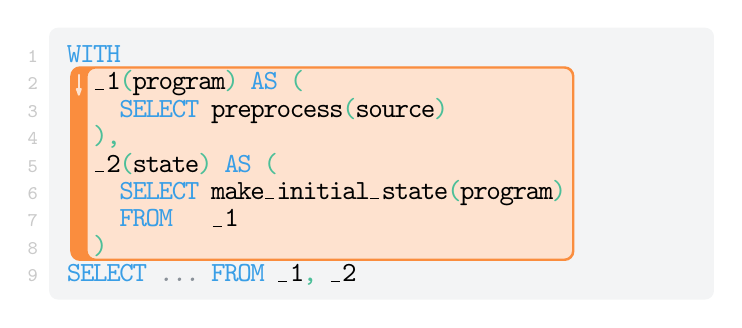
\begin{tikzpicture}[x=1.1ex,y=-2.3ex]
      \begin{scope}[%
        inner sep=0mm,outer sep=0mm,%
        every node/.style={anchor=text,font=\color{codeForeground}\ttfamily\mdseries},%
        keyword/.style={font=\color{codeKeyword}\ttfamily\bfseries},%
        builtin/.style={font=\color{codeBuiltin}\ttfamily\bfseries},%
        constant/.style={font=\color{codeConstant}\ttfamily},%
        operator/.style={font=\color{codeOperator}\ttfamily},%
        emph/.style={font=\color{codeEmph}\ttfamily\bfseries},%
        string/.style={font=\color{codeString}\ttfamily\mdseries},%
        comment/.style={font=\color{codeComment}\ttfamily\itshape},%
        linenum/.style={font=\color{codeRuler}\smaller[2]\ttfamily}%
      ]
        % WITH
        \node[linenum ] at (-3, 0) {1};
        \node[keyword ] at ( 0, 0) (firstline) {W};
        \node[keyword ] at ( 1, 0) {I};
        \node[keyword ] at ( 2, 0) {T};
        \node[keyword ] at ( 3, 0) {H};
        %   _1(program) AS (
        \node[linenum ] at (-3, 1) {2};
        \node[        ] at ( 2, 1) {\_};
        \node[        ] at ( 3, 1) {1};
        \node[operator] at ( 4, 1) {(};
        \node[        ] at ( 5, 1) {p};
        \node[        ] at ( 6, 1) {r};
        \node[        ] at ( 7, 1) {o};
        \node[        ] at ( 8, 1) {g};
        \node[        ] at ( 9, 1) {r};
        \node[        ] at (10, 1) {a};
        \node[        ] at (11, 1) {m};
        \node[operator] at (12, 1) {)};
        \node[keyword ] at (14, 1) {A};
        \node[keyword ] at (15, 1) {S};
        \node[operator] at (17, 1) (firstlinear) {(};
        %     SELECT preprocess(source)
        \node[linenum ] at (-3, 2) {3};
        \node[keyword ] at ( 4, 2) {S};
        \node[keyword ] at ( 5, 2) {E};
        \node[keyword ] at ( 6, 2) {L};
        \node[keyword ] at ( 7, 2) {E};
        \node[keyword ] at ( 8, 2) {C};
        \node[keyword ] at ( 9, 2) {T};
        \node[        ] at (11, 2) {p};
        \node[        ] at (12, 2) {r};
        \node[        ] at (13, 2) {e};
        \node[        ] at (14, 2) {p};
        \node[        ] at (15, 2) {r};
        \node[        ] at (16, 2) {o};
        \node[        ] at (17, 2) {c};
        \node[        ] at (18, 2) {e};
        \node[        ] at (19, 2) {s};
        \node[        ] at (20, 2) {s};
        \node[operator] at (21, 2) {(};
        \node[        ] at (22, 2) {s};
        \node[        ] at (23, 2) {o};
        \node[        ] at (24, 2) {u};
        \node[        ] at (25, 2) {r};
        \node[        ] at (26, 2) {c};
        \node[        ] at (27, 2) {e};
        \node[operator] at (28, 2) {)};
        %   ),
        \node[linenum ] at (-3, 3) {4};
        \node[operator] at ( 2, 3) {)};
        \node[operator] at ( 3, 3) {,};
        %   _2(state) AS (
        \node[linenum ] at (-3, 4) {5};
        \node[        ] at ( 2, 4) {\_};
        \node[        ] at ( 3, 4) {2};
        \node[operator] at ( 4, 4) {(};
        \node[        ] at ( 5, 4) {s};
        \node[        ] at ( 6, 4) {t};
        \node[        ] at ( 7, 4) {a};
        \node[        ] at ( 8, 4) {t};
        \node[        ] at ( 9, 4) {e};
        \node[operator] at (10, 4) {)};
        \node[keyword ] at (12, 4) {A};
        \node[keyword ] at (13, 4) {S};
        \node[operator] at (15, 4) {(};
        %     SELECT make_inital_state(program)
        \node[linenum ] at (-3, 5) {6};
        \node[keyword ] at ( 4, 5) {S};
        \node[keyword ] at ( 5, 5) {E};
        \node[keyword ] at ( 6, 5) {L};
        \node[keyword ] at ( 7, 5) {E};
        \node[keyword ] at ( 8, 5) {C};
        \node[keyword ] at ( 9, 5) {T};
        \node[        ] at (11, 5) {m};
        \node[        ] at (12, 5) {a};
        \node[        ] at (13, 5) {k};
        \node[        ] at (14, 5) {e};
        \node[        ] at (15, 5) {\_};
        \node[        ] at (16, 5) {i};
        \node[        ] at (17, 5) {n};
        \node[        ] at (18, 5) {i};
        \node[        ] at (19, 5) {t};
        \node[        ] at (20, 5) {i};
        \node[        ] at (21, 5) {a};
        \node[        ] at (22, 5) {l};
        \node[        ] at (23, 5) {\_};
        \node[        ] at (24, 5) {s};
        \node[        ] at (25, 5) {t};
        \node[        ] at (26, 5) {a};
        \node[        ] at (27, 5) {t};
        \node[        ] at (28, 5) {e};
        \node[operator] at (29, 5) {(};
        \node[        ] at (30, 5) {p};
        \node[        ] at (31, 5) {r};
        \node[        ] at (32, 5) {o};
        \node[        ] at (33, 5) {g};
        \node[        ] at (34, 5) {r};
        \node[        ] at (35, 5) {a};
        \node[        ] at (36, 5) {m};
        \node[operator] at (37, 5) (longestline) {)};
        %     FROM   _1
        \node[linenum ] at (-3, 6) {7};
        \node[keyword ] at ( 4, 6) {F};
        \node[keyword ] at ( 5, 6) {R};
        \node[keyword ] at ( 6, 6) {O};
        \node[keyword ] at ( 7, 6) {M};
        \node[        ] at (11, 6) {\_};
        \node[        ] at (12, 6) {1};
        %   )
        \node[linenum ] at (-3, 7) {8};
        \node[operator] at ( 2, 7) (lastlinear) {)};
        % SELECT ... FROM _1, _2
        \node[linenum ] at (-3, 8) {9};
        \node[keyword ] at ( 0, 8) {S};
        \node[keyword ] at ( 1, 8) {E};
        \node[keyword ] at ( 2, 8) {L};
        \node[keyword ] at ( 3, 8) {E};
        \node[keyword ] at ( 4, 8) {C};
        \node[keyword ] at ( 5, 8) {T};
        \node[comment ] at ( 7, 8) {.};
        \node[comment ] at ( 8, 8) {.};
        \node[comment ] at ( 9, 8) {.};
        \node[keyword ] at (11, 8) (lastline) {F};
        \node[keyword ] at (12, 8) {R};
        \node[keyword ] at (13, 8) {O};
        \node[keyword ] at (14, 8) {M};
        \node[        ] at (16, 8) {\_};
        \node[        ] at (17, 8) {1};
        \node[operator] at (18, 8) {,};
        \node[        ] at (20, 8) {\_};
        \node[        ] at (21, 8) {2};
      \end{scope}
      \begin{pgfonlayer}{background}
        \coordinate (extent) at (48,0);
        \begin{scope}[%
          rounded corners=0.75ex,%
          inner sep=0pt,%
          background/.style={fill=codebg,inner xsep=1.5ex, inner ysep=1.5ex},
          dummy bounding box/.style={inner xsep=0.5ex, inner ysep=0.2ex},%
          bounding box/.style={inner sep=0pt, line width=0.15ex},%
          dummy annotation/.style={anchor=center,outer sep=0.3ex},%
          annotation/.style={anchor=center},%
          dummy decoration/.style={inner sep=0.3ex},%
          decoration/.style={line width=0.15ex},%
        ]
          \node[dummy bounding box,fit=(firstlinear) (lastlinear) (longestline)] (linear) {};
          \node[dummy annotation] at ($(linear.north west) + (-0.6,0.7)$) (arr) {\linearCFarrow{}};
          \node[fit=(linear) (arr)] (_linear) {};

          \node[background,fit=(firstline) (lastline) (_linear) (extent)] {};
          \node[bounding box, draw=linear, fill=linear   , fit=(_linear)] {};
          \node[bounding box, draw=linear, fill=linear!25, fit=(linear) ] {};
          \node[annotation, linear!25] at (arr.center) {\linearCFarrow{}};
        \end{scope}
      \end{pgfonlayer}
    \end{tikzpicture}
    \caption{\cfoption{linear}{1} Consecutive CTEs}
    \label{fig:linear-control-flow-sql-cte}
  \end{subfigure}
  \begin{subfigure}{0.4\textwidth}
    \centering
    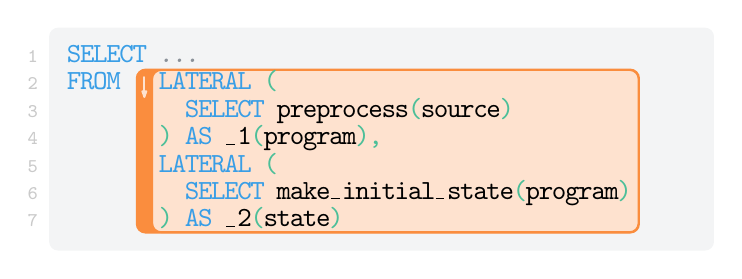
\begin{tikzpicture}[x=1.1ex,y=-2.3ex]
      \begin{scope}[%
        inner sep=0mm,outer sep=0mm,%
        every node/.style={anchor=text,font=\color{codeForeground}\ttfamily\mdseries},%
        keyword/.style={font=\color{codeKeyword}\ttfamily\bfseries},%
        builtin/.style={font=\color{codeBuiltin}\ttfamily\bfseries},%
        constant/.style={font=\color{codeConstant}\ttfamily},%
        operator/.style={font=\color{codeOperator}\ttfamily},%
        emph/.style={font=\color{codeEmph}\ttfamily\bfseries},%
        string/.style={font=\color{codeString}\ttfamily\mdseries},%
        comment/.style={font=\color{codeComment}\ttfamily\itshape},%
        linenum/.style={font=\color{codeRuler}\smaller[2]\ttfamily}%
      ]
        % SELECT ...
        \node[linenum ] at (-3, 0) {1};
        \node[keyword ] at ( 0, 0) (firstline) {S};
        \node[keyword ] at ( 1, 0) {E};
        \node[keyword ] at ( 2, 0) {L};
        \node[keyword ] at ( 3, 0) {E};
        \node[keyword ] at ( 4, 0) {C};
        \node[keyword ] at ( 5, 0) {T};
        \node[comment ] at ( 7, 0) {.};
        \node[comment ] at ( 8, 0) {.};
        \node[comment ] at ( 9, 0) {.};
        % FROM   LATERAL (
        \node[linenum ] at (-3, 1) {2};
        \node[keyword ] at ( 0, 1) {F};
        \node[keyword ] at ( 1, 1) {R};
        \node[keyword ] at ( 2, 1) {O};
        \node[keyword ] at ( 3, 1) {M};
        \node[keyword ] at ( 7, 1) (firstlinear) {L};
        \node[keyword ] at ( 8, 1) {A};
        \node[keyword ] at ( 9, 1) {T};
        \node[keyword ] at (10, 1) {E};
        \node[keyword ] at (11, 1) {R};
        \node[keyword ] at (12, 1) {A};
        \node[keyword ] at (13, 1) {L};
        \node[operator] at (15, 1) {(};
        %          SELECT preprocess(source)
        \node[linenum ] at (-3, 2) {3};
        \node[keyword ] at ( 9, 2) {S};
        \node[keyword ] at (10, 2) {E};
        \node[keyword ] at (11, 2) {L};
        \node[keyword ] at (12, 2) {E};
        \node[keyword ] at (13, 2) {C};
        \node[keyword ] at (14, 2) {T};
        \node[        ] at (16, 2) {p};
        \node[        ] at (17, 2) {r};
        \node[        ] at (18, 2) {e};
        \node[        ] at (19, 2) {p};
        \node[        ] at (20, 2) {r};
        \node[        ] at (21, 2) {o};
        \node[        ] at (22, 2) {c};
        \node[        ] at (23, 2) {e};
        \node[        ] at (24, 2) {s};
        \node[        ] at (25, 2) {s};
        \node[operator] at (26, 2) {(};
        \node[        ] at (27, 2) {s};
        \node[        ] at (28, 2) {o};
        \node[        ] at (29, 2) {u};
        \node[        ] at (30, 2) {r};
        \node[        ] at (31, 2) {c};
        \node[        ] at (32, 2) {e};
        \node[operator] at (33, 2) {)};
        %        ) AS _1(program),
        \node[linenum ] at (-3, 3) {4};
        \node[operator] at ( 7, 3) {)};
        \node[keyword ] at ( 9, 3) {A};
        \node[keyword ] at (10, 3) {S};
        \node[        ] at (12, 3) {\_};
        \node[        ] at (13, 3) {1};
        \node[operator] at (14, 3) {(};
        \node[        ] at (15, 3) {p};
        \node[        ] at (16, 3) {r};
        \node[        ] at (17, 3) {o};
        \node[        ] at (18, 3) {g};
        \node[        ] at (19, 3) {r};
        \node[        ] at (20, 3) {a};
        \node[        ] at (21, 3) {m};
        \node[operator] at (22, 3) {)};
        \node[operator] at (23, 3) {,};
        %        LATERAL (
        \node[linenum ] at (-3, 4) {5};
        \node[keyword ] at ( 7, 4) {L};
        \node[keyword ] at ( 8, 4) {A};
        \node[keyword ] at ( 9, 4) {T};
        \node[keyword ] at (10, 4) {E};
        \node[keyword ] at (11, 4) {R};
        \node[keyword ] at (12, 4) {A};
        \node[keyword ] at (13, 4) {L};
        \node[operator] at (15, 4) {(};
        %           SELECT make_inital_state(program)
        \node[linenum ] at (-3, 5) {6};
        \node[keyword ] at ( 9, 5) {S};
        \node[keyword ] at (10, 5) {E};
        \node[keyword ] at (11, 5) {L};
        \node[keyword ] at (12, 5) {E};
        \node[keyword ] at (13, 5) {C};
        \node[keyword ] at (14, 5) {T};
        \node[        ] at (16, 5) {m};
        \node[        ] at (17, 5) {a};
        \node[        ] at (18, 5) {k};
        \node[        ] at (19, 5) {e};
        \node[        ] at (20, 5) {\_};
        \node[        ] at (21, 5) {i};
        \node[        ] at (22, 5) {n};
        \node[        ] at (23, 5) {i};
        \node[        ] at (24, 5) {t};
        \node[        ] at (25, 5) {i};
        \node[        ] at (26, 5) {a};
        \node[        ] at (27, 5) {l};
        \node[        ] at (28, 5) {\_};
        \node[        ] at (29, 5) {s};
        \node[        ] at (30, 5) {t};
        \node[        ] at (31, 5) {a};
        \node[        ] at (32, 5) {t};
        \node[        ] at (33, 5) {e};
        \node[operator] at (34, 5) {(};
        \node[        ] at (35, 5) {p};
        \node[        ] at (36, 5) {r};
        \node[        ] at (37, 5) {o};
        \node[        ] at (38, 5) {g};
        \node[        ] at (39, 5) {r};
        \node[        ] at (40, 5) {a};
        \node[        ] at (41, 5) {m};
        \node[operator] at (42, 5) (longestline) {)};
        %        ) AS _2(state)
        \node[linenum ] at (-3, 6) {7};
        \node[operator] at ( 7, 6) {)};
        \node[keyword ] at ( 9, 6) {A};
        \node[keyword ] at (10, 6) {S};
        \node[        ] at (12, 6) {\_};
        \node[        ] at (13, 6) {2};
        \node[operator] at (14, 6) (lastline) {(};
        \node[        ] at (15, 6) {s};
        \node[        ] at (16, 6) {t};
        \node[        ] at (17, 6) {a};
        \node[        ] at (18, 6) {t};
        \node[        ] at (19, 6) {e};
        \node[operator] at (20, 6) (lastlinear) {)};
      \end{scope}
      \begin{pgfonlayer}{background}
        \coordinate (extent) at (48,0);
        \begin{scope}[%
          rounded corners=0.75ex,%
          inner sep=0pt,%
          background/.style={fill=codebg,inner xsep=1.5ex, inner ysep=1.5ex},
          dummy bounding box/.style={inner xsep=0.5ex, inner ysep=0.2ex},%
          bounding box/.style={inner sep=0pt, line width=0.15ex},%
          dummy annotation/.style={anchor=center,outer sep=0.3ex},%
          annotation/.style={anchor=center},%
          dummy decoration/.style={inner sep=0.3ex},%
          decoration/.style={line width=0.15ex},%
        ]
          \node[dummy bounding box,fit=(firstlinear) (lastlinear) (longestline)] (linear) {};
          \node[dummy annotation] at ($(linear.north west) + (-0.6,0.7)$) (arr) {\linearCFarrow{}};
          \node[fit=(linear) (arr)] (_linear) {};

          \node[background,fit=(firstline) (lastline) (_linear) (extent)] {};
          \node[bounding box, draw=linear, fill=linear   , fit=(_linear)] {};
          \node[bounding box, draw=linear, fill=linear!25, fit=(linear) ] {};
          \node[annotation, linear!25] at (arr.center) {\linearCFarrow{}};
        \end{scope}
      \end{pgfonlayer}
    \end{tikzpicture}
    \caption{\cfoption{linear}{2} Consecutive \keyword{LATERAL}-Joins}
    \label{fig:linear-control-flow-sql-lateral}
  \end{subfigure}
  \begin{subfigure}{0.4\textwidth}
    \centering
    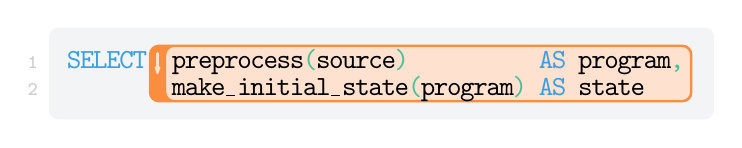
\begin{tikzpicture}[x=1.1ex,y=-2.3ex]
      \begin{scope}[%
        inner sep=0mm,outer sep=0mm,%
        every node/.style={anchor=text,font=\color{codeForeground}\ttfamily\mdseries},%
        keyword/.style={font=\color{codeKeyword}\ttfamily\bfseries},%
        builtin/.style={font=\color{codeBuiltin}\ttfamily\bfseries},%
        constant/.style={font=\color{codeConstant}\ttfamily},%
        operator/.style={font=\color{codeOperator}\ttfamily},%
        emph/.style={font=\color{codeEmph}\ttfamily\bfseries},%
        string/.style={font=\color{codeString}\ttfamily\mdseries},%
        comment/.style={font=\color{codeComment}\ttfamily\itshape},%
        linenum/.style={font=\color{codeRuler}\smaller[2]\ttfamily}%
      ]
        % SELECT preprocess(source) AS program,
        \node[linenum ] at (-3, 0) {1};
        \node[keyword ] at ( 0, 0) (firstline) {S};
        \node[keyword ] at ( 1, 0) {E};
        \node[keyword ] at ( 2, 0) {L};
        \node[keyword ] at ( 3, 0) {E};
        \node[keyword ] at ( 4, 0) {C};
        \node[keyword ] at ( 5, 0) {T};
        \node[        ] at ( 8, 0) {p};
        \node[        ] at ( 9, 0) {r};
        \node[        ] at (10, 0) {e};
        \node[        ] at (11, 0) {p};
        \node[        ] at (12, 0) {r};
        \node[        ] at (13, 0) {o};
        \node[        ] at (14, 0) {c};
        \node[        ] at (15, 0) {e};
        \node[        ] at (16, 0) {s};
        \node[        ] at (17, 0) {s};
        \node[operator] at (18, 0) (firstlinear) {(};
        \node[        ] at (19, 0) {s};
        \node[        ] at (20, 0) {o};
        \node[        ] at (21, 0) {u};
        \node[        ] at (22, 0) {r};
        \node[        ] at (23, 0) {c};
        \node[        ] at (24, 0) {e};
        \node[operator] at (25, 0) {)};
        \node[keyword ] at (36, 0) {A};
        \node[keyword ] at (37, 0) {S};
        \node[        ] at (39, 0) {p};
        \node[        ] at (40, 0) {r};
        \node[        ] at (41, 0) {o};
        \node[        ] at (42, 0) {g};
        \node[        ] at (43, 0) {r};
        \node[        ] at (44, 0) {a};
        \node[        ] at (45, 0) {m};
        \node[operator] at (46, 0) (longestline) {,};
        %        make_inital_state(program) AS state
        \node[linenum ] at (-3, 1) {2};
        \node[        ] at ( 8, 1) (lastlinear) {m};
        \node[        ] at ( 9, 1) {a};
        \node[        ] at ( 10, 1) {k};
        \node[        ] at (11, 1) {e};
        \node[        ] at (12, 1) {\_};
        \node[        ] at (13, 1) {i};
        \node[        ] at (14, 1) {n};
        \node[        ] at (15, 1) {i};
        \node[        ] at (16, 1) {t};
        \node[        ] at (17, 1) {i};
        \node[        ] at (18, 1) {a};
        \node[        ] at (19, 1) {l};
        \node[        ] at (20, 1) {\_};
        \node[        ] at (21, 1) {s};
        \node[        ] at (22, 1) {t};
        \node[        ] at (23, 1) {a};
        \node[        ] at (24, 1) {t};
        \node[        ] at (25, 1) {e};
        \node[operator] at (26, 1) {(};
        \node[        ] at (27, 1) {p};
        \node[        ] at (28, 1) {r};
        \node[        ] at (29, 1) {o};
        \node[        ] at (30, 1) {g};
        \node[        ] at (31, 1) {r};
        \node[        ] at (32, 1) {a};
        \node[        ] at (33, 1) {m};
        \node[operator] at (34, 1) (lastline) {)};
        \node[keyword ] at (36, 1) {A};
        \node[keyword ] at (37, 1) {S};
        \node[        ] at (39, 1) {s};
        \node[        ] at (40, 1) {t};
        \node[        ] at (41, 1) {a};
        \node[        ] at (42, 1) {t};
        \node[        ] at (43, 1) {e};
      \end{scope}
      \begin{pgfonlayer}{background}
        \coordinate (extent) at (48,0);
        \begin{scope}[%
          rounded corners=0.75ex,%
          inner sep=0pt,%
          background/.style={fill=codebg,inner xsep=1.5ex, inner ysep=1.5ex},
          dummy bounding box/.style={inner xsep=0.5ex, inner ysep=0.2ex},%
          bounding box/.style={inner sep=0pt, line width=0.15ex},%
          dummy annotation/.style={anchor=center,outer sep=0.3ex},%
          annotation/.style={anchor=center},%
          dummy decoration/.style={inner sep=0.3ex},%
          decoration/.style={line width=0.15ex},%
        ]
          \node[dummy bounding box,fit=(firstlinear) (lastline) (lastlinear) (longestline)] (linear) {};
          \node[dummy annotation] at ($(linear.north west) + (-0.6,0.7)$) (arr) {\linearCFarrow{}};
          \node[fit=(linear) (arr)] (_linear) {};

          \node[background,fit=(firstline) (lastline) (_linear) (extent)] {};
          \node[bounding box, draw=linear, fill=linear   , fit=(_linear)] {};
          \node[bounding box, draw=linear, fill=linear!25, fit=(linear) ] {};
          \node[annotation, linear!25] at (arr.center) {\linearCFarrow{}};
        \end{scope}
      \end{pgfonlayer}
    \end{tikzpicture}
    \caption{\cfoption{linear}{3} Left-Looking Column-Alias-References}
    \label{fig:linear-control-flow-sql-select}
  \end{subfigure}
  \caption{{\color{linear}Linear} control flow in multiple representations in SQL.}
  \label{fig:linear-control-flow-sql}
\end{figure}

There are multiple options to represent straight-line control flow in SQL, we
will go through the pros, cons, and availability of three of these.

\begin{enumerate}
  \item[\cfoption{linear}{1}] The first option is to chain the
   individual statements in the linear sequence as individual common table
   expressions(CTEs)---as illustrated in \Cref
   {fig:linear-control-flow-sql-cte}. Most developers know of this technique as
   it is the go-to way to decompose complex queries into simpler constituent
   parts.

  \item[\cfoption{linear}{2}] The second option is to make use
   of \keyword{LATERAL}-joins---as illustrated in \Cref
   {fig:linear-control-flow-sql-lateral}. These allow query authors to use row
   and column variables inside a table expression from other table expressions
   preceding it in the same \keyword{FROM}-clause.

  \item[\cfoption{linear}{3}]The last option is to use left-looking
   column-alias-references; a non-standard feature not available in many
   RDBMS---as illustrated in \Cref{fig:linear-control-flow-sql-select}. It
   allows for \keyword{LATERAL}-esque references to preceding expressions in
   the projection list of a \keyword{SELECT}-clause.
\end{enumerate}

From a purely ergonomic perspective \cfoption{linear}{3} left-looking
column-alias-references win by a long shot. Sadly, few large RDBMSs support
them as they are a non-standard feature. Additionally, in most implementations,
there are limitations as to what expressions can be referenced. For example, in
DuckDB \cite{duckdb} one can only reference aliases bound to what they call
``simple expressions''---for example, this excludes subqueries.

Both \cfoption{linear}{1} CTEs and \cfoption{linear}{2} \keyword
{LATERAL}-joins are equally supported by a very wide set of RDBMSs. There are
multiple factors at play when choosing one over the other. For example,
depending on how performant your RDBMS of choice implements CTEs there may be
performance benefits or drawbacks over \keyword{LATERAL}-joins. In this paper,
we will make use of the \keyword{LATERAL}-join variant due to how it interacts
with the translations of the other two control flow types.

\subsection{\usebox{\branchingCFbox}\ Branching Control Flow}
\label{sec:branching-cf}

\begin{figure}[t]
  \centering
  \begin{subfigure}{0.20\textwidth}
    \centering
    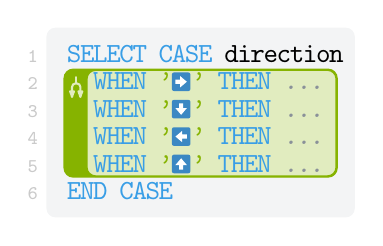
\begin{tikzpicture}[x=1.1ex,y=-2.3ex]
      \begin{scope}[%
        inner sep=0mm,outer sep=0mm,%
        every node/.style={anchor=text,font=\color{codeForeground}\ttfamily\mdseries},%
        keyword/.style={font=\color{codeKeyword}\ttfamily\bfseries},%
        builtin/.style={font=\color{codeBuiltin}\ttfamily\bfseries},%
        constant/.style={font=\color{codeConstant}\ttfamily},%
        operator/.style={font=\color{codeOperator}\ttfamily},%
        emph/.style={font=\color{codeEmph}\ttfamily\bfseries},%
        string/.style={font=\color{codeString}\ttfamily\mdseries},%
        comment/.style={font=\color{codeComment}\ttfamily\itshape},%
        linenum/.style={font=\color{codeRuler}\smaller[2]\ttfamily}%
      ]
        % SELECT CASE direction
        \node[linenum ] at (-3, 0) {1};
        \node[keyword ] at ( 0, 0) (firstline) {S};
        \node[keyword ] at ( 1, 0) {E};
        \node[keyword ] at ( 2, 0) {L};
        \node[keyword ] at ( 3, 0) {E};
        \node[keyword ] at ( 4, 0) {C};
        \node[keyword ] at ( 5, 0) {T};
        \node[keyword ] at ( 7, 0) {C};
        \node[keyword ] at ( 8, 0) {A};
        \node[keyword ] at ( 9, 0) {S};
        \node[keyword ] at (10, 0) {E};
        \node[        ] at (12, 0) {d};
        \node[        ] at (13, 0) {i};
        \node[        ] at (14, 0) {r};
        \node[        ] at (15, 0) {e};
        \node[        ] at (16, 0) {c};
        \node[        ] at (17, 0) {t};
        \node[        ] at (18, 0) {i};
        \node[        ] at (19, 0) {o};
        \node[        ] at (20, 0) {n};
        %   WHEN '' THEN ...
        \node[linenum ] at (-3, 1) {2};
        \node[keyword ] at ( 2, 1) (firstbranching) {W};
        \node[keyword ] at ( 3, 1) {H};
        \node[keyword ] at ( 4, 1) {E};
        \node[keyword ] at ( 5, 1) {N};
        \node[string  ] at ( 7, 1) {\verb|'|};
        \node[string  ] at ( 8, 1) {\texttwemoji{right arrow}};
        \node[string  ] at ( 9.5, 1) {\verb|'|};
        \node[keyword ] at (11.5, 1) {T};
        \node[keyword ] at (12.5, 1) {H};
        \node[keyword ] at (13.5, 1) {E};
        \node[keyword ] at (14.5, 1) {N};
        \node[comment ] at (16.5, 1) {.};
        \node[comment ] at (17.5, 1) {.};
        \node[comment ] at (18.5, 1) (longestline) {.};
        %   WHEN '' THEN ...
        \node[linenum ] at (-3, 2) {3};
        \node[keyword ] at ( 2, 2) {W};
        \node[keyword ] at ( 3, 2) {H};
        \node[keyword ] at ( 4, 2) {E};
        \node[keyword ] at ( 5, 2) {N};
        \node[string  ] at ( 7, 2) {\verb|'|};
        \node[string  ] at ( 8, 2) {\texttwemoji{down arrow}};
        \node[string  ] at ( 9.5, 2) {\verb|'|};
        \node[keyword ] at (11.5, 2) {T};
        \node[keyword ] at (12.5, 2) {H};
        \node[keyword ] at (13.5, 2) {E};
        \node[keyword ] at (14.5, 2) {N};
        \node[comment ] at (16.5, 2) {.};
        \node[comment ] at (17.5, 2) {.};
        \node[comment ] at (18.5, 2) {.};
        %   WHEN '' THEN ...
        \node[linenum ] at (-3, 3) {4};
        \node[keyword ] at ( 2, 3) {W};
        \node[keyword ] at ( 3, 3) {H};
        \node[keyword ] at ( 4, 3) {E};
        \node[keyword ] at ( 5, 3) {N};
        \node[string  ] at ( 7, 3) {\verb|'|};
        \node[string  ] at ( 8, 3) {\texttwemoji{left arrow}};
        \node[string  ] at ( 9.5, 3) {\verb|'|};
        \node[keyword ] at (11.5, 3) {T};
        \node[keyword ] at (12.5, 3) {H};
        \node[keyword ] at (13.5, 3) {E};
        \node[keyword ] at (14.5, 3) {N};
        \node[comment ] at (16.5, 3) {.};
        \node[comment ] at (17.5, 3) {.};
        \node[comment ] at (18.5, 3) {.};
        %   WHEN '' THEN ...
        \node[linenum ] at (-3, 4) {5};
        \node[keyword ] at ( 2, 4) {W};
        \node[keyword ] at ( 3, 4) {H};
        \node[keyword ] at ( 4, 4) {E};
        \node[keyword ] at ( 5, 4) {N};
        \node[string  ] at ( 7, 4) {\verb|'|};
        \node[string  ] at ( 8, 4) (lastbranching) {\texttwemoji{up arrow}};
        \node[string  ] at ( 9.5, 4) {\verb|'|};
        \node[keyword ] at (11.5, 4) {T};
        \node[keyword ] at (12.5, 4) {H};
        \node[keyword ] at (13.5, 4) {E};
        \node[keyword ] at (14.5, 4) {N};
        \node[comment ] at (16.5, 4) {.};
        \node[comment ] at (17.5, 4) {.};
        \node[comment ] at (18.5, 4) {.};
        % END
        \node[linenum ] at (-3, 5) {6};
        \node[keyword ] at ( 0, 5) (lastline) {E};
        \node[keyword ] at ( 1, 5) {N};
        \node[keyword ] at ( 2, 5) {D};
        \node[keyword ] at ( 4, 5) {C};
        \node[keyword ] at ( 5, 5) {A};
        \node[keyword ] at ( 6, 5) {S};
        \node[keyword ] at ( 7, 5) {E};
      \end{scope}
      \begin{pgfonlayer}{background}
        \begin{scope}[%
          rounded corners=0.75ex,%
          inner sep=0pt,%
          background/.style={fill=codebg,inner xsep=1.5ex, inner ysep=1.5ex},
          dummy bounding box/.style={inner xsep=0.5ex, inner ysep=0.2ex},%
          bounding box/.style={inner sep=0pt, line width=0.15ex},%
          dummy annotation/.style={anchor=center,outer sep=0.3ex},%
          annotation/.style={anchor=center},%
        ]
          \coordinate (extent) at ($(longestline)+(1,0)$);
          \node[dummy bounding box,fit=(firstbranching) (lastbranching) (extent)] (branching) {};
          \node[dummy annotation] at ($(branching.north west) + (-0.8,0.7)$) (arr) {\branchingCFarrow{}};
          \node[fit=(branching) (arr)] (_branching) {};

          \node[background,fit=(firstline) (lastline) (_branching)] {};
          \node[bounding box, draw=branching, fill=branching   , fit=(_branching)] {};
          \node[bounding box, draw=branching, fill=branching!25, fit=(branching) ] {};
          \node[annotation, branching!25] at (arr.center) {\branchingCFarrow{}};
        \end{scope}
      \end{pgfonlayer}
    \end{tikzpicture}
    \caption{\cfoption{branching}{1} \keyword{CASE} Expressions}
    \label{fig:branching-control-flow-sql-case}
  \end{subfigure}%
  \hfill%
  \begin{subfigure}{0.24\textwidth}
    \centering
    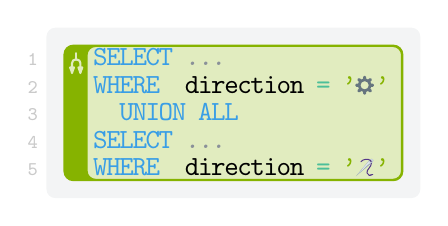
\begin{tikzpicture}[x=1.1ex,y=-2.3ex]
      \begin{scope}[%
        inner sep=0mm,outer sep=0mm,%
        every node/.style={anchor=text,font=\color{codeForeground}\ttfamily\mdseries},%
        keyword/.style={font=\color{codeKeyword}\ttfamily\bfseries},%
        builtin/.style={font=\color{codeBuiltin}\ttfamily\bfseries},%
        constant/.style={font=\color{codeConstant}\ttfamily},%
        operator/.style={font=\color{codeOperator}\ttfamily\bfseries},%
        emph/.style={font=\color{codeEmph}\ttfamily\bfseries},%
        string/.style={font=\color{codeString}\ttfamily},%
        comment/.style={font=\color{codeComment}\ttfamily\itshape},%
        linenum/.style={font=\color{codeRuler}\smaller[2]\ttfamily}%
      ]
        % SELECT ...
        \node[linenum ] at (-3, 0) {1};
        \node[keyword ] at ( 2, 0) (firstbranching) {S};
        \node[keyword ] at ( 3, 0) (firstline) {E};
        \node[keyword ] at ( 4, 0) {L};
        \node[keyword ] at ( 5, 0) {E};
        \node[keyword ] at ( 6, 0) {C};
        \node[keyword ] at ( 7, 0) {T};
        \node[comment ] at ( 9, 0) {.};
        \node[comment ] at ( 10, 0) {.};
        \node[comment ] at ( 11, 0) {.};
        % WHERE  mode=''
        \node[linenum ] at (-3, 1) {2};
        \node[keyword ] at ( 2, 1) {W};
        \node[keyword ] at ( 3, 1) {H};
        \node[keyword ] at ( 4, 1) {E};
        \node[keyword ] at ( 5, 1) {R};
        \node[keyword ] at ( 6, 1) {E};
        \node[        ] at ( 9, 1) {d};
        \node[        ] at ( 10, 1) {i};
        \node[        ] at ( 11, 1) {r};
        \node[        ] at (12, 1) {e};
        \node[        ] at (13, 1) {c};
        \node[        ] at (14, 1) {t};
        \node[        ] at (15, 1) {i};
        \node[        ] at (16, 1) {o};
        \node[        ] at (17, 1) {n};
        \node[operator] at (19, 1) {=};
        \node[string  ] at (21, 1) {\verb|'|};
        \node[        ] at (22, 1) {\texttwemoji{gear}};
        \node[string  ] at (23.5, 1) (longestline) {\verb|'|};
        %   UNION ALL
        \node[linenum ] at (-3, 2) {3};
        \node[keyword ] at ( 4, 2) {U};
        \node[keyword ] at ( 5, 2) {N};
        \node[keyword ] at ( 6, 2) {I};
        \node[keyword ] at ( 7, 2) {O};
        \node[keyword ] at ( 8, 2) {N};
        \node[keyword ] at (10, 2) {A};
        \node[keyword ] at (11, 2) {L};
        \node[keyword ] at (12, 2) {L};
        % SELECT ...
        \node[linenum ] at (-3, 3) {4};
        \node[keyword ] at ( 2, 3) {S};
        \node[keyword ] at ( 3, 3) {E};
        \node[keyword ] at ( 4, 3) {L};
        \node[keyword ] at ( 5, 3) {E};
        \node[keyword ] at ( 6, 3) {C};
        \node[keyword ] at ( 7, 3) {T};
        \node[comment ] at ( 9, 3) {.};
        \node[comment ] at (10, 3) {.};
        \node[comment ] at (11, 3) {.};
        % WHERE  mode=''
        \node[linenum ] at (-3, 4) {5};
        \node[keyword ] at ( 2, 4) (lastline) {W};
        \node[keyword ] at ( 3, 4) {H};
        \node[keyword ] at ( 4, 4) {E};
        \node[keyword ] at ( 5, 4) {R};
        \node[keyword ] at ( 6, 4) {E};
        \node[        ] at ( 9, 4) {d};
        \node[        ] at (10, 4) {i};
        \node[        ] at (11, 4) {r};
        \node[        ] at (12, 4) {e};
        \node[        ] at (13, 4) {c};
        \node[        ] at (14, 4) {t};
        \node[        ] at (15, 4) {i};
        \node[        ] at (16, 4) {o};
        \node[        ] at (17, 4) {n};
        \node[operator] at (19, 4) {=};
        \node[string  ] at (21, 4) {\verb|'|};
        \node[        ] at (22, 4) (lastbranching) {\texttwemoji{sewing needle}};
        \node[string  ] at (23.5,4) {\verb|'|};
      \end{scope}
      \begin{pgfonlayer}{background}
        \begin{scope}[%
          rounded corners=0.75ex,%
          inner sep=0pt,%
          background/.style={fill=codebg,inner xsep=1.5ex, inner ysep=1.5ex},
          dummy bounding box/.style={inner xsep=0.5ex, inner ysep=0.2ex},%
          bounding box/.style={inner sep=0pt, line width=0.15ex},%
          dummy annotation/.style={anchor=center,outer sep=0.3ex},%
          annotation/.style={anchor=center},%
        ]
          \coordinate (extent) at ($(longestline)+(1,0)$);
          \node[dummy bounding box,fit=(firstbranching) (lastbranching) (extent)] (branching) {};
          \node[dummy annotation] at ($(branching.north west) + (-0.8,0.7)$) (arr) {\branchingCFarrow{}};
          \node[fit=(branching) (arr)] (_branching) {};

          \node[background,fit=(firstline) (lastline) (_branching)] {};
          \node[bounding box, draw=branching, fill=branching   , fit=(_branching)] {};
          \node[bounding box, draw=branching, fill=branching!25, fit=(branching) ] {};
          \node[annotation, branching!25] at (arr.center) {\branchingCFarrow{}};
        \end{scope}
      \end{pgfonlayer}
    \end{tikzpicture}
    \caption{\cfoption{branching}{2} Mutually Distinct \keyword{UNION ALL}}
    \label{fig:branching-control-flow-sql-union}
  \end{subfigure}
  \caption{{\color{branching}Branching} control flow in multiple representations in SQL.}
  \label{fig:branching-control-flow-sql}
\end{figure}

SQL provides two options for representing branching behavior, one using SQL's
expression language and one using SQL's relational design.

\begin{enumerate}
  \item[\cfoption{branching}{1}] SQL's expression language offers branching
   control flow in the form of \keyword{CASE}-expressions as in \Cref
   {fig:branching-control-flow-sql-case}.

  \item[\cfoption{branching}{2}] Aside from the direct option, pure relational
   algebra can represent conditional evaluation as well. Inheriting from set
   theory, mutually distinct unions, as illustrated in \Cref
   {fig:branching-control-flow-sql-union}, allow for expression of ``optional
   execution''.
\end{enumerate}

Though the more direct solution of the two, \cfoption{branching}{1} \keyword
{CASE}-expressions come with some difficulties depending on the targeted
RDBMSs. The type-checking/-inference systems of some RDBMSs are weak and
require type annotations. Some of these type systems do not support the ad-hoc
generation of complex types in scalar positions, e.g., row types with named
columns.

When trying to make things work out with \keyword{CASE}-expressions while
skirting around the type system limitations, one option is to ``push down''
the \keyword{CASE} to each scalar value. But this leads to subpar performance
in most RDBMSs. In contrast, RDBMSs are exceptional at performing relational
workloads like computing \cfoption{branching}{2} mutually distinct unions. Some
RDBMSs optimize such workloads in such a manner that the ``lazy'' behavior of
branching control flow is retained.

\subsection{\usebox{\nonlinearCFbox}\ Looping Control Flow}
\label{sec:non-linear-cf}

\begin{figure}[t]
  \centering
  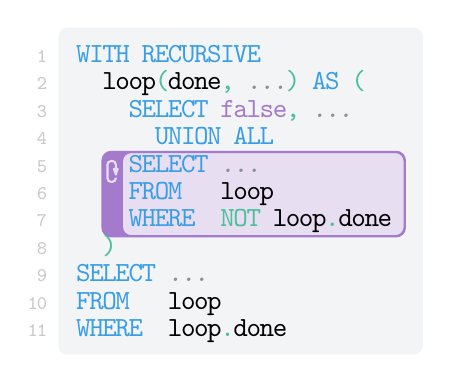
\begin{tikzpicture}[x=1.1ex,y=-2.3ex]
    \begin{scope}[%
      inner sep=0mm,outer sep=0mm,%
      every node/.style={anchor=text,font=\color{codeForeground}\ttfamily\mdseries},%
      keyword/.style={font=\color{codeKeyword}\ttfamily\bfseries},%
      builtin/.style={font=\color{codeBuiltin}\ttfamily\bfseries},%
      constant/.style={font=\color{codeConstant}\ttfamily},%
      operator/.style={font=\color{codeOperator}\ttfamily},%
      emph/.style={font=\color{codeEmph}\ttfamily\bfseries},%
      string/.style={font=\color{codeString}\ttfamily\mdseries},%
      comment/.style={font=\color{codeComment}\ttfamily\itshape},%
      linenum/.style={font=\color{codeRuler}\smaller[2]\ttfamily}%
    ]
      % WITH RECURSIVE
      \node[linenum ] at (-3, 0) {1};
      \node[keyword ] at ( 0, 0) (firstline) {W};
      \node[keyword ] at ( 1, 0) {I};
      \node[keyword ] at ( 2, 0) {T};
      \node[keyword ] at ( 3, 0) {H};
      \node[keyword ] at ( 5, 0) {R};
      \node[keyword ] at ( 6, 0) {E};
      \node[keyword ] at ( 7, 0) {C};
      \node[keyword ] at ( 8, 0) {U};
      \node[keyword ] at ( 9, 0) {R};
      \node[keyword ] at (10, 0) {S};
      \node[keyword ] at (11, 0) {I};
      \node[keyword ] at (12, 0) {V};
      \node[keyword ] at (13, 0) {E};
      %   loop(done, ...) AS (
      \node[linenum ] at (-3, 1) {2};
      \node[        ] at ( 2, 1) {l};
      \node[        ] at ( 3, 1) {o};
      \node[        ] at ( 4, 1) {o};
      \node[        ] at ( 5, 1) {p};
      \node[operator] at ( 6, 1) {(};
      \node[        ] at ( 7, 1) {d};
      \node[        ] at ( 8, 1) {o};
      \node[        ] at ( 9, 1) {n};
      \node[        ] at (10, 1) {e};
      \node[operator] at (11, 1) {,};
      \node[comment ] at (13, 1) {.};
      \node[comment ] at (14, 1) {.};
      \node[comment ] at (15, 1) {.};
      \node[operator] at (16, 1) {)};
      \node[keyword ] at (18, 1) {A};
      \node[keyword ] at (19, 1) {S};
      \node[operator] at (21, 1) {(};
      %     SELECT false, ...
      \node[linenum ] at (-3, 2) {3};
      \node[keyword ] at ( 4, 2) {S};
      \node[keyword ] at ( 5, 2) {E};
      \node[keyword ] at ( 6, 2) {L};
      \node[keyword ] at ( 7, 2) {E};
      \node[keyword ] at ( 8, 2) {C};
      \node[keyword ] at ( 9, 2) {T};
      \node[constant] at (11, 2) {f};
      \node[constant] at (12, 2) {a};
      \node[constant] at (13, 2) {l};
      \node[constant] at (14, 2) {s};
      \node[constant] at (15, 2) {e};
      \node[operator] at (16, 2) {,};
      \node[comment ] at (18, 2) {.};
      \node[comment ] at (19, 2) {.};
      \node[comment ] at (20, 2) {.};
      %       UNION ALL
      \node[linenum ] at (-3, 3) {4};
      \node[keyword ] at ( 6, 3) {U};
      \node[keyword ] at ( 7, 3) {N};
      \node[keyword ] at ( 8, 3) {I};
      \node[keyword ] at ( 9, 3) {O};
      \node[keyword ] at (10, 3) {N};
      \node[keyword ] at (12, 3) {A};
      \node[keyword ] at (13, 3) {L};
      \node[keyword ] at (14, 3) {L};
      %     SELECT ...
      \node[linenum ] at (-3, 4) {5};
      \node[keyword ] at ( 4, 4) (firstnonlinear) {S};
      \node[keyword ] at ( 5, 4) {E};
      \node[keyword ] at ( 6, 4) {L};
      \node[keyword ] at ( 7, 4) {E};
      \node[keyword ] at ( 8, 4) {C};
      \node[keyword ] at ( 9, 4) {T};
      \node[comment ] at (11, 4) {.};
      \node[comment ] at (12, 4) {.};
      \node[comment ] at (13, 4) {.};
      %     FROM   loop
      \node[linenum ] at (-3, 5) {6};
      \node[keyword ] at ( 4, 5) {F};
      \node[keyword ] at ( 5, 5) {R};
      \node[keyword ] at ( 6, 5) {O};
      \node[keyword ] at ( 7, 5) {M};
      \node[        ] at (11, 5) {l};
      \node[        ] at (12, 5) {o};
      \node[        ] at (13, 5) {o};
      \node[        ] at (14, 5) {p};
      %     WHERE  NOT loop.done
      \node[linenum ] at (-3, 6) {7};
      \node[keyword ] at ( 4, 6) {W};
      \node[keyword ] at ( 5, 6) {H};
      \node[keyword ] at ( 6, 6) {E};
      \node[keyword ] at ( 7, 6) {R};
      \node[keyword ] at ( 8, 6) {E};
      \node[operator] at (11, 6) {N};
      \node[operator] at (12, 6) {O};
      \node[operator] at (13, 6) {T};
      \node[        ] at (15, 6) {l};
      \node[        ] at (16, 6) {o};
      \node[        ] at (17, 6) {o};
      \node[        ] at (18, 6) (lastnonlinear) {p};
      \node[operator] at (19, 6) {.};
      \node[        ] at (20, 6) {d};
      \node[        ] at (21, 6) {o};
      \node[        ] at (22, 6) {n};
      \node[        ] at (23, 6) (longestline) {e};
      %   )
      \node[linenum ] at (-3, 7) {8};
      \node[operator] at ( 2, 7) {)};
      % SELECT ...
      \node[linenum ] at (-3, 8) {9};
      \node[keyword ] at ( 0, 8) {S};
      \node[keyword ] at ( 1, 8) {E};
      \node[keyword ] at ( 2, 8) {L};
      \node[keyword ] at ( 3, 8) {E};
      \node[keyword ] at ( 4, 8) {C};
      \node[keyword ] at ( 5, 8) {T};
      \node[comment] at ( 7, 8) {.};
      \node[comment] at ( 8, 8) {.};
      \node[comment] at ( 9, 8) {.};
      % FROM   loop
      \node[linenum ] at (-3.7, 9) {1};
      \node[linenum ] at (-3, 9) {0};
      \node[keyword ] at ( 0, 9) {F};
      \node[keyword ] at ( 1, 9) {R};
      \node[keyword ] at ( 2, 9) {O};
      \node[keyword ] at ( 3, 9) {M};
      \node[        ] at ( 7, 9) {l};
      \node[        ] at ( 8, 9) {o};
      \node[        ] at ( 9, 9) {o};
      \node[        ] at (10, 9) {p};
      % WHERE  loop.done
      \node[linenum ] at (-3.7,10) {1};
      \node[linenum ] at (-3,10) {1};
      \node[keyword ] at ( 0,10) (lastline) {W};
      \node[keyword ] at ( 1,10) {H};
      \node[keyword ] at ( 2,10) {E};
      \node[keyword ] at ( 3,10) {R};
      \node[keyword ] at ( 4,10) {E};
      \node[        ] at ( 7,10) {l};
      \node[        ] at ( 8,10) {o};
      \node[        ] at ( 9,10) {o};
      \node[        ] at (10,10) {p};
      \node[operator] at (11,10) {.};
      \node[        ] at (12,10) {d};
      \node[        ] at (13,10) {o};
      \node[        ] at (14,10) {n};
      \node[        ] at (15,10) {e};
    \end{scope}
    \begin{pgfonlayer}{background}
      \begin{scope}[%
        rounded corners=0.75ex,%
        inner sep=0pt,%
        background/.style={fill=codebg,inner xsep=1.5ex, inner ysep=1.5ex},
        dummy bounding box/.style={inner xsep=0.5ex, inner ysep=0.2ex},%
        bounding box/.style={inner sep=0pt, line width=0.15ex},%
        dummy annotation/.style={anchor=center,outer sep=0.3ex},%
        annotation/.style={anchor=center},%
      ]
        \coordinate (extent) at ($(longestline)+(1,0)$);
        \node[dummy bounding box,fit=(firstnonlinear) (lastnonlinear) (extent)] (nonlinear) {};
        \node[dummy annotation] at ($(nonlinear.north west) + (-0.7,0.7)$) (arr) {\nonlinearCFarrow{}};
        \node[fit=(nonlinear) (arr)] (_nonlinear) {};

        \node[background,fit=(firstline) (lastline) (_nonlinear)] {};
        \node[bounding box, draw=nonlinear, fill=nonlinear   , fit=(_nonlinear)] {};
        \node[bounding box, draw=nonlinear, fill=nonlinear!25, fit=(nonlinear) ] {};
        \node[annotation, nonlinear!25] at (arr.center) {\nonlinearCFarrow{}};
      \end{scope}
    \end{pgfonlayer}
  \end{tikzpicture}
  \caption{{\color{nonlinear}Looping} control flow represented through a
   recursive CTE \mbox{(i.e., \keyword{WITH RECURSIVE})}.}
  \label{fig:non-linear-control-flow-sql}
\end{figure}

In contrast to the previous two types of control flow, looping control flow
requires Turing completeness and there is only one SQL:1999 option for Turing
completeness in SQL: \keyword{WITH RECURSIVE}. Recursive CTEs consist of two
distinct parts, the base case and the recursive term. Starting from the base
case the recursive term is iteratively applied to the previously produced rows.
This iterative application is performed until no rows are produced, at which
point the rows produced during each iteration are considered the result of the
CTE.

Due to \keyword{WITH RECURSIVE}s bare-bone semantics, the only directly
equivalent loops are \keyword{do}-\keyword{while}-loops. As such, translating
all other loop constructs starts with translating them into \keyword
{do}-\keyword{while}-notation. This usually entails adding extra control data
like indexes or flags to the local program state.

There are some performance considerations to take into account when translating
imperative loops to SQL. Depending on how your underlying RDBMS keeps track of
the rows the individual iterations produce, a lot of data may need to be copied
around in memory. A slight remedy for these performance pains is to keep
loop-invariant and transient data out of the working table.

\subsection{Putting It All Together}

\begin{figure}[t]
  \centering
  \smaller
  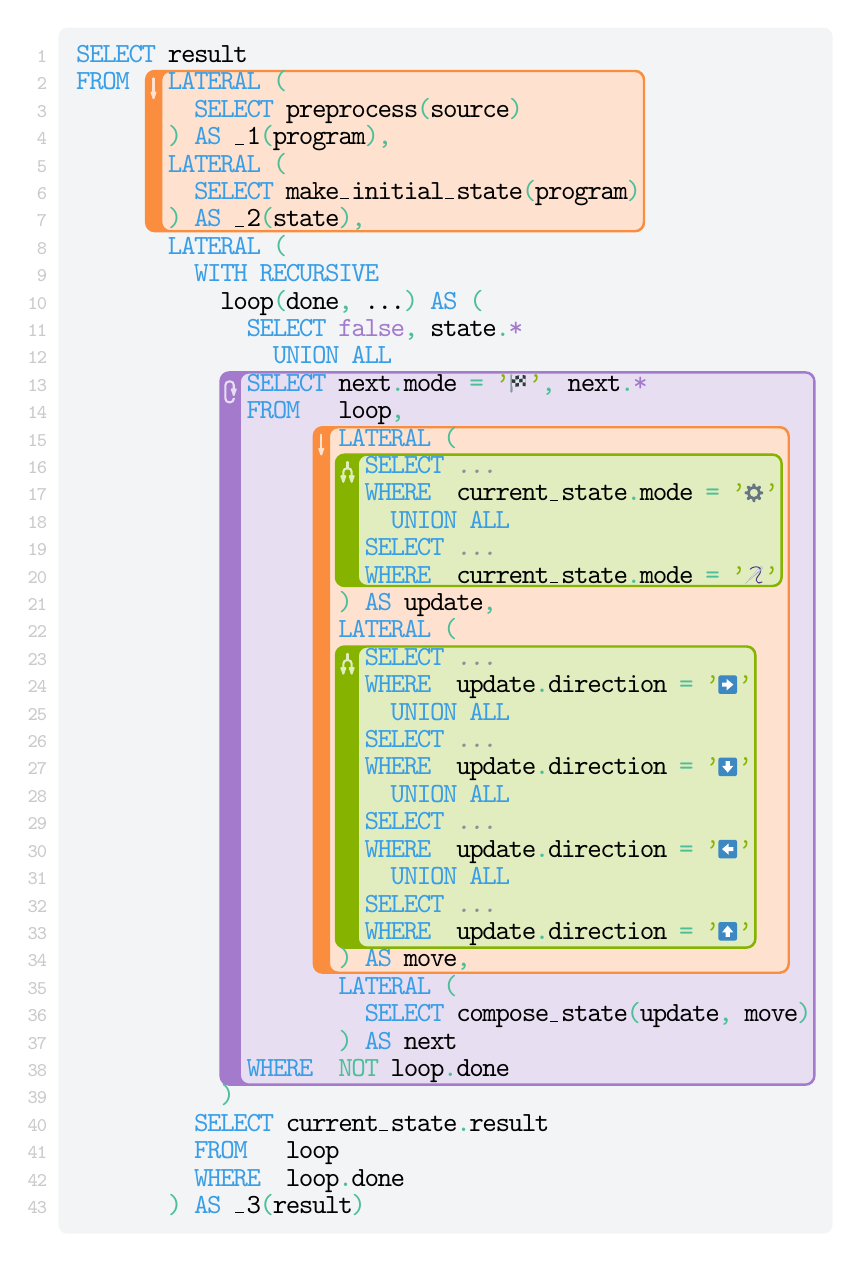
\begin{tikzpicture}[x=1.1ex,y=-2.3ex]
    \begin{scope}[%
      inner sep=0mm,outer sep=0mm,%
      every node/.style={anchor=text,font=\color{codeForeground}\ttfamily\mdseries},%
      keyword/.style={font=\color{codeKeyword}\ttfamily\bfseries},%
      builtin/.style={font=\color{codeBuiltin}\ttfamily\bfseries},%
      constant/.style={font=\color{codeConstant}\ttfamily},%
      operator/.style={font=\color{codeOperator}\ttfamily},%
      emph/.style={font=\color{codeEmph}\ttfamily\bfseries},%
      string/.style={font=\color{codeString}\ttfamily\mdseries},%
      comment/.style={font=\color{codeComment}\ttfamily\itshape},%
      linenum/.style={font=\color{codeRuler}\smaller[2]\ttfamily}%
    ]
      % SELECT result
      \node[linenum ] at (-3, 0) {1};
      \node[keyword ] at ( 0, 0) (firstline) {S};
      \node[keyword ] at ( 1, 0) {E};
      \node[keyword ] at ( 2, 0) {L};
      \node[keyword ] at ( 3, 0) {E};
      \node[keyword ] at ( 4, 0) {C};
      \node[keyword ] at ( 5, 0) {T};
      \node[        ] at ( 7, 0) {r};
      \node[        ] at ( 8, 0) {e};
      \node[        ] at ( 9, 0) {s};
      \node[        ] at (10, 0) {u};
      \node[        ] at (11, 0) {l};
      \node[        ] at (12, 0) {t};
      % FROM   LATERAL (
      \node[linenum ] at (-3, 1) {2};
      \node[keyword ] at ( 0, 1) {F};
      \node[keyword ] at ( 1, 1) {R};
      \node[keyword ] at ( 2, 1) {O};
      \node[keyword ] at ( 3, 1) {M};
      \node[keyword ] at ( 7, 1) (firstsetup) {L};
      \node[keyword ] at ( 8, 1) {A};
      \node[keyword ] at ( 9, 1) {T};
      \node[keyword ] at (10, 1) {E};
      \node[keyword ] at (11, 1) {R};
      \node[keyword ] at (12, 1) {A};
      \node[keyword ] at (13, 1) {L};
      \node[operator] at (15, 1) {(};
      %          SELECT preprocess(source)
      \node[linenum ] at (-3, 2) {3};
      \node[keyword ] at ( 9, 2) {S};
      \node[keyword ] at (10, 2) {E};
      \node[keyword ] at (11, 2) {L};
      \node[keyword ] at (12, 2) {E};
      \node[keyword ] at (13, 2) {C};
      \node[keyword ] at (14, 2) {T};
      \node[        ] at (16, 2) {p};
      \node[        ] at (17, 2) {r};
      \node[        ] at (18, 2) {e};
      \node[        ] at (19, 2) {p};
      \node[        ] at (20, 2) {r};
      \node[        ] at (21, 2) {o};
      \node[        ] at (22, 2) {c};
      \node[        ] at (23, 2) {e};
      \node[        ] at (24, 2) {s};
      \node[        ] at (25, 2) {s};
      \node[operator] at (26, 2) {(};
      \node[        ] at (27, 2) {s};
      \node[        ] at (28, 2) {o};
      \node[        ] at (29, 2) {u};
      \node[        ] at (30, 2) {r};
      \node[        ] at (31, 2) {c};
      \node[        ] at (32, 2) {e};
      \node[operator] at (33, 2) {)};
      %        ) AS _1(program),
      \node[linenum ] at (-3, 3) {4};
      \node[operator] at ( 7, 3) {)};
      \node[keyword ] at ( 9, 3) {A};
      \node[keyword ] at (10, 3) {S};
      \node[        ] at (12, 3) {\_};
      \node[        ] at (13, 3) {1};
      \node[operator] at (14, 3) {(};
      \node[        ] at (15, 3) {p};
      \node[        ] at (16, 3) {r};
      \node[        ] at (17, 3) {o};
      \node[        ] at (18, 3) {g};
      \node[        ] at (19, 3) {r};
      \node[        ] at (20, 3) {a};
      \node[        ] at (21, 3) {m};
      \node[operator] at (22, 3) {)};
      \node[operator] at (23, 3) {,};
      %        LATERAL (
      \node[linenum ] at (-3, 4) {5};
      \node[keyword ] at ( 7, 4) {L};
      \node[keyword ] at ( 8, 4) {A};
      \node[keyword ] at ( 9, 4) {T};
      \node[keyword ] at (10, 4) {E};
      \node[keyword ] at (11, 4) {R};
      \node[keyword ] at (12, 4) {A};
      \node[keyword ] at (13, 4) {L};
      \node[operator] at (15, 4) {(};
      %          SELECT make_initial_state(program)
      \node[linenum ] at (-3, 5) {6};
      \node[keyword ] at ( 9, 5) {S};
      \node[keyword ] at (10, 5) {E};
      \node[keyword ] at (11, 5) {L};
      \node[keyword ] at (12, 5) {E};
      \node[keyword ] at (13, 5) {C};
      \node[keyword ] at (14, 5) {T};
      \node[        ] at (16, 5) {m};
      \node[        ] at (17, 5) {a};
      \node[        ] at (18, 5) {k};
      \node[        ] at (19, 5) {e};
      \node[        ] at (20, 5) {\_};
      \node[        ] at (21, 5) {i};
      \node[        ] at (22, 5) {n};
      \node[        ] at (23, 5) {i};
      \node[        ] at (24, 5) {t};
      \node[        ] at (25, 5) {i};
      \node[        ] at (26, 5) {a};
      \node[        ] at (27, 5) {l};
      \node[        ] at (28, 5) {\_};
      \node[        ] at (29, 5) {s};
      \node[        ] at (30, 5) {t};
      \node[        ] at (31, 5) {a};
      \node[        ] at (32, 5) {t};
      \node[        ] at (33, 5) {e};
      \node[operator] at (34, 5) {(};
      \node[        ] at (35, 5) {p};
      \node[        ] at (36, 5) {r};
      \node[        ] at (37, 5) {o};
      \node[        ] at (38, 5) {g};
      \node[        ] at (39, 5) {r};
      \node[        ] at (40, 5) {a};
      \node[        ] at (41, 5) {m};
      \node[operator] at (42, 5) (longestsetup) {)};
      %        ) AS _2(state),
      \node[linenum ] at (-3, 6) {7};
      \node[operator] at ( 7, 6) (lastsetup) {)};
      \node[keyword ] at ( 9, 6) {A};
      \node[keyword ] at (10, 6) {S};
      \node[        ] at (12, 6) {\_};
      \node[        ] at (13, 6) {2};
      \node[operator] at (14, 6) {(};
      \node[        ] at (15, 6) {s};
      \node[        ] at (16, 6) {t};
      \node[        ] at (17, 6) {a};
      \node[        ] at (18, 6) {t};
      \node[        ] at (19, 6) {e};
      \node[operator] at (20, 6) {)};
      \node[operator] at (21, 6) {,};
      %        LATERAL (
      \node[linenum ] at (-3, 7) {8};
      \node[keyword ] at ( 7, 7) {L};
      \node[keyword ] at ( 8, 7) {A};
      \node[keyword ] at ( 9, 7) {T};
      \node[keyword ] at (10, 7) {E};
      \node[keyword ] at (11, 7) {R};
      \node[keyword ] at (12, 7) {A};
      \node[keyword ] at (13, 7) {L};
      \node[operator] at (15, 7) {(};
      %          WITH RECURSIVE
      \node[linenum ] at (-3, 8) {9};
      \node[keyword ] at ( 9, 8) {W};
      \node[keyword ] at (10, 8) {I};
      \node[keyword ] at (11, 8) {T};
      \node[keyword ] at (12, 8) {H};
      \node[keyword ] at (14, 8) {R};
      \node[keyword ] at (15, 8) {E};
      \node[keyword ] at (16, 8) {C};
      \node[keyword ] at (17, 8) {U};
      \node[keyword ] at (18, 8) {R};
      \node[keyword ] at (19, 8) {S};
      \node[keyword ] at (20, 8) {I};
      \node[keyword ] at (21, 8) {V};
      \node[keyword ] at (22, 8) {E};
      %            loop(done, ...) AS (
      \node[linenum ] at (-3.7, 9) {1};
      \node[linenum ] at (-3, 9) {0};
      \node[        ] at (11, 9) {l};
      \node[        ] at (12, 9) {o};
      \node[        ] at (13, 9) {o};
      \node[        ] at (14, 9) {p};
      \node[operator] at (15, 9) {(};
      \node[        ] at (16, 9) {d};
      \node[        ] at (17, 9) {o};
      \node[        ] at (18, 9) {n};
      \node[        ] at (19, 9) {e};
      \node[operator] at (20, 9) {,};
      \node[        ] at (22, 9) {.};
      \node[        ] at (23, 9) {.};
      \node[        ] at (24, 9) {.};
      \node[operator] at (25, 9) {)};
      \node[keyword ] at (27, 9) {A};
      \node[keyword ] at (28, 9) {S};
      \node[operator] at (30, 9) {(};
      %              SELECT false, state.*
      \node[linenum ] at (-3.7,10) {1};
      \node[linenum ] at (-3,10) {1};
      \node[keyword ] at (13,10) {S};
      \node[keyword ] at (14,10) {E};
      \node[keyword ] at (15,10) {L};
      \node[keyword ] at (16,10) {E};
      \node[keyword ] at (17,10) {C};
      \node[keyword ] at (18,10) {T};
      \node[constant] at (20,10) {f};
      \node[constant] at (21,10) {a};
      \node[constant] at (22,10) {l};
      \node[constant] at (23,10) {s};
      \node[constant] at (24,10) {e};
      \node[operator] at (25,10) {,};
      \node[        ] at (27,10) {s};
      \node[        ] at (28,10) {t};
      \node[        ] at (29,10) {a};
      \node[        ] at (30,10) {t};
      \node[        ] at (31,10) {e};
      \node[operator] at (32,10) {.};
      \node[constant] at (33,10) {*};
      %                UNION ALL
      \node[linenum ] at (-3.7,11) {1};
      \node[linenum ] at (-3,11) {2};
      \node[keyword ] at (15,11) {U};
      \node[keyword ] at (16,11) {N};
      \node[keyword ] at (17,11) {I};
      \node[keyword ] at (18,11) {O};
      \node[keyword ] at (19,11) {N};
      \node[keyword ] at (21,11) {A};
      \node[keyword ] at (22,11) {L};
      \node[keyword ] at (23,11) {L};
      %              SELECT next.mode = '🏁', next.*
      \node[linenum ] at (-3.7,12) {1};
      \node[linenum ] at (-3,12) {3};
      \node[keyword ] at (13,12) (firstnonlinear) {S};
      \node[keyword ] at (14,12) {E};
      \node[keyword ] at (15,12) {L};
      \node[keyword ] at (16,12) {E};
      \node[keyword ] at (17,12) {C};
      \node[keyword ] at (18,12) {T};
      \node[        ] at (20,12) {n};
      \node[        ] at (21,12) {e};
      \node[        ] at (22,12) {x};
      \node[        ] at (23,12) {t};
      \node[operator] at (24,12) {.};
      \node[        ] at (25,12) {m};
      \node[        ] at (26,12) {o};
      \node[        ] at (27,12) {d};
      \node[        ] at (28,12) {e};
      \node[operator] at (30,12) {=};
      \node[string  ] at (32,12) (_firstnonlinear) {\verb|'|};
      \node[        ] at (33,12) {\texttwemoji{chequered flag}};
      \node[string  ] at (34.5,12) {\verb|'|};
      \node[operator] at (35.5,12) {,};
      \node[        ] at (37.5,12) {n};
      \node[        ] at (38.5,12) {e};
      \node[        ] at (39.5,12) {x};
      \node[        ] at (40.5,12) {t};
      \node[operator] at (41.5,12) {.};
      \node[constant] at (42.5,12) {*};
      %              FROM   loop,
      \node[linenum ] at (-3.7,13) {1};
      \node[linenum ] at (-3,13) {4};
      \node[keyword ] at (13,13) {F};
      \node[keyword ] at (14,13) {R};
      \node[keyword ] at (15,13) {O};
      \node[keyword ] at (16,13) {M};
      \node[        ] at (20,13) {l};
      \node[        ] at (21,13) {o};
      \node[        ] at (22,13) {o};
      \node[        ] at (23,13) {p};
      \node[operator] at (24,13) {,};
      %                     LATERAL (
      \node[linenum ] at (-3.7,14) {1};
      \node[linenum ] at (-3,14) {5};
      \node[keyword ] at (20,14) (firstbody) {L};
      \node[keyword ] at (21,14) {A};
      \node[keyword ] at (22,14) {T};
      \node[keyword ] at (23,14) {E};
      \node[keyword ] at (24,14) {R};
      \node[keyword ] at (25,14) {A};
      \node[keyword ] at (26,14) {L};
      \node[operator] at (28,14) {(};
      %                       SELECT ...
      \node[linenum ] at (-3.7,15) {1};
      \node[linenum ] at (-3,15) {6};
      \node[keyword ] at (22,15) (firstmodebranch) {S};
      \node[keyword ] at (23,15) {E};
      \node[keyword ] at (24,15) {L};
      \node[keyword ] at (25,15) {E};
      \node[keyword ] at (26,15) {C};
      \node[keyword ] at (27,15) {T};
      \node[comment ] at (29,15) {.};
      \node[comment ] at (30,15) {.};
      \node[comment ] at (31,15) {.};
      %                       WHERE  current_state.mode = '⚙'
      \node[linenum ] at (-3.7,16) {1};
      \node[linenum ] at (-3,16) {7};
      \node[keyword ] at (22,16) {W};
      \node[keyword ] at (23,16) {H};
      \node[keyword ] at (24,16) {E};
      \node[keyword ] at (25,16) {R};
      \node[keyword ] at (26,16) {E};
      \node[        ] at (29,16) {c};
      \node[        ] at (30,16) {u};
      \node[        ] at (31,16) {r};
      \node[        ] at (32,16) {r};
      \node[        ] at (33,16) {e};
      \node[        ] at (34,16) {n};
      \node[        ] at (35,16) {t};
      \node[        ] at (36,16) {\_};
      \node[        ] at (37,16) {s};
      \node[        ] at (38,16) {t};
      \node[        ] at (39,16) {a};
      \node[        ] at (40,16) {t};
      \node[        ] at (41,16) {e};
      \node[operator] at (42,16) {.};
      \node[        ] at (43,16) {m};
      \node[        ] at (44,16) {o};
      \node[        ] at (45,16) {d};
      \node[        ] at (46,16) {e};
      \node[operator] at (48,16) {=};
      \node[string  ] at (50,16) {\verb|'|};
      \node[        ] at (51,16) {\texttwemoji{gear}};
      \node[string  ] at (52.5,16) (longestmodebranch) {\verb|'|};
      %                         UNION ALL
      \node[linenum ] at (-3.7,17) {1};
      \node[linenum ] at (-3,17) {8};
      \node[keyword ] at (24,17) {U};
      \node[keyword ] at (25,17) {N};
      \node[keyword ] at (26,17) {I};
      \node[keyword ] at (27,17) {O};
      \node[keyword ] at (28,17) {N};
      \node[keyword ] at (30,17) {A};
      \node[keyword ] at (31,17) {L};
      \node[keyword ] at (32,17) {L};
      %                       SELECT ...
      \node[linenum ] at (-3.7,18) {1};
      \node[linenum ] at (-3,18) {9};
      \node[keyword ] at (22,18) {S};
      \node[keyword ] at (23,18) {E};
      \node[keyword ] at (24,18) {L};
      \node[keyword ] at (25,18) {E};
      \node[keyword ] at (26,18) {C};
      \node[keyword ] at (27,18) {T};
      \node[comment ] at (29,18) {.};
      \node[comment ] at (30,18) {.};
      \node[comment ] at (31,18) {.};
      %                       WHERE  current_state.mode = '🪡'
      \node[linenum ] at (-3.7,19) {2};
      \node[linenum ] at (-3,19) {0};
      \node[keyword ] at (22,19) {W};
      \node[keyword ] at (23,19) {H};
      \node[keyword ] at (24,19) {E};
      \node[keyword ] at (25,19) {R};
      \node[keyword ] at (26,19) {E};
      \node[        ] at (29,19) {c};
      \node[        ] at (30,19) {u};
      \node[        ] at (31,19) {r};
      \node[        ] at (32,19) {r};
      \node[        ] at (33,19) {e};
      \node[        ] at (34,19) {n};
      \node[        ] at (35,19) {t};
      \node[        ] at (36,19) (lastmodebranch) {\_};
      \node[        ] at (37,19) {s};
      \node[        ] at (38,19) {t};
      \node[        ] at (39,19) {a};
      \node[        ] at (40,19) {t};
      \node[        ] at (41,19) {e};
      \node[operator] at (42,19) {.};
      \node[        ] at (43,19) {m};
      \node[        ] at (44,19) {o};
      \node[        ] at (45,19) {d};
      \node[        ] at (46,19) {e};
      \node[operator] at (48,19) {=};
      \node[string  ] at (50,19) {\verb|'|};
      \node[        ] at (51,19) {\texttwemoji{sewing needle}};
      \node[string  ] at (52.5,19) {\verb|'|};
      %                     ) AS update,
      \node[linenum ] at (-3.7,20) {2};
      \node[linenum ] at (-3,20) {1};
      \node[operator] at (20,20) {)};
      \node[keyword ] at (22,20) {A};
      \node[keyword ] at (23,20) {S};
      \node[        ] at (25,20) {u};
      \node[        ] at (26,20) {p};
      \node[        ] at (27,20) {d};
      \node[        ] at (28,20) {a};
      \node[        ] at (29,20) {t};
      \node[        ] at (30,20) {e};
      \node[operator] at (31,20) {,};
      %                     LATERAL (
      \node[linenum ] at (-3.7,21) {2};
      \node[linenum ] at (-3,21) {2};
      \node[keyword ] at (20,21) {L};
      \node[keyword ] at (21,21) {A};
      \node[keyword ] at (22,21) {T};
      \node[keyword ] at (23,21) {E};
      \node[keyword ] at (24,21) {R};
      \node[keyword ] at (25,21) {A};
      \node[keyword ] at (26,21) {L};
      \node[operator] at (28,21) {(};
      %                       SELECT ...
      \node[linenum ] at (-3.7,22) {2};
      \node[linenum ] at (-3,22) {3};
      \node[keyword ] at (22,22) (firstdirbranch) {S};
      \node[keyword ] at (23,22) {E};
      \node[keyword ] at (24,22) {L};
      \node[keyword ] at (25,22) {E};
      \node[keyword ] at (26,22) {C};
      \node[keyword ] at (27,22) {T};
      \node[comment ] at (29,22) {.};
      \node[comment ] at (30,22) {.};
      \node[comment ] at (31,22) {.};
      %                       WHERE  update.direction = '➡️'
      \node[linenum ] at (-3.7,23) {2};
      \node[linenum ] at (-3,23) {4};
      \node[keyword ] at (22,23) {W};
      \node[keyword ] at (23,23) {H};
      \node[keyword ] at (24,23) {E};
      \node[keyword ] at (25,23) {R};
      \node[keyword ] at (26,23) {E};
      \node[        ] at (29,23) {u};
      \node[        ] at (30,23) {p};
      \node[        ] at (31,23) {d};
      \node[        ] at (32,23) {a};
      \node[        ] at (33,23) {t};
      \node[        ] at (34,23) {e};
      \node[operator] at (35,23) {.};
      \node[        ] at (36,23) {d};
      \node[        ] at (37,23) {i};
      \node[        ] at (38,23) {r};
      \node[        ] at (39,23) {e};
      \node[        ] at (40,23) {c};
      \node[        ] at (41,23) {t};
      \node[        ] at (42,23) {i};
      \node[        ] at (43,23) {o};
      \node[        ] at (44,23) {n};
      \node[operator] at (46,23) {=};
      \node[string  ] at (48,23) {\verb|'|};
      \node[        ] at (49,23) {\texttwemoji{right arrow}};
      \node[string  ] at (50.5,23) (longestdirbranch) {\verb|'|};
      %                         UNION ALL
      \node[linenum ] at (-3.7,24) {2};
      \node[linenum ] at (-3,24) {5};
      \node[keyword ] at (24,24) {U};
      \node[keyword ] at (25,24) {N};
      \node[keyword ] at (26,24) {I};
      \node[keyword ] at (27,24) {O};
      \node[keyword ] at (28,24) {N};
      \node[keyword ] at (30,24) {A};
      \node[keyword ] at (31,24) {L};
      \node[keyword ] at (32,24) {L};
      %                       SELECT ...
      \node[linenum ] at (-3.7,25) {2};
      \node[linenum ] at (-3,25) {6};
      \node[keyword ] at (22,25) {S};
      \node[keyword ] at (23,25) {E};
      \node[keyword ] at (24,25) {L};
      \node[keyword ] at (25,25) {E};
      \node[keyword ] at (26,25) {C};
      \node[keyword ] at (27,25) {T};
      \node[comment ] at (29,25) {.};
      \node[comment ] at (30,25) {.};
      \node[comment ] at (31,25) {.};
      %                       WHERE  update.direction = '⬇️'
      \node[linenum ] at (-3.7,26) {2};
      \node[linenum ] at (-3,26) {7};
      \node[keyword ] at (22,26) {W};
      \node[keyword ] at (23,26) {H};
      \node[keyword ] at (24,26) {E};
      \node[keyword ] at (25,26) {R};
      \node[keyword ] at (26,26) {E};
      \node[        ] at (29,26) {u};
      \node[        ] at (30,26) {p};
      \node[        ] at (31,26) {d};
      \node[        ] at (32,26) {a};
      \node[        ] at (33,26) {t};
      \node[        ] at (34,26) {e};
      \node[operator] at (35,26) {.};
      \node[        ] at (36,26) {d};
      \node[        ] at (37,26) {i};
      \node[        ] at (38,26) {r};
      \node[        ] at (39,26) {e};
      \node[        ] at (40,26) {c};
      \node[        ] at (41,26) {t};
      \node[        ] at (42,26) {i};
      \node[        ] at (43,26) {o};
      \node[        ] at (44,26) {n};
      \node[operator] at (46,26) {=};
      \node[string  ] at (48,26) {\verb|'|};
      \node[        ] at (49,26) {\texttwemoji{down arrow}};
      \node[string  ] at (50.5,26) {\verb|'|};
      %                         UNION ALL
      \node[linenum ] at (-3.7,27) {2};
      \node[linenum ] at (-3,27) {8};
      \node[keyword ] at (24,27) {U};
      \node[keyword ] at (25,27) {N};
      \node[keyword ] at (26,27) {I};
      \node[keyword ] at (27,27) {O};
      \node[keyword ] at (28,27) {N};
      \node[keyword ] at (30,27) {A};
      \node[keyword ] at (31,27) {L};
      \node[keyword ] at (32,27) {L};
      %                       SELECT ...
      \node[linenum ] at (-3.7,28) {2};
      \node[linenum ] at (-3,28) {9};
      \node[keyword ] at (22,28) {S};
      \node[keyword ] at (23,28) {E};
      \node[keyword ] at (24,28) {L};
      \node[keyword ] at (25,28) {E};
      \node[keyword ] at (26,28) {C};
      \node[keyword ] at (27,28) {T};
      \node[comment ] at (29,28) {.};
      \node[comment ] at (30,28) {.};
      \node[comment ] at (31,28) {.};
      %                       WHERE  update.direction = '⬅️'
      \node[linenum ] at (-3.7,29) {3};
      \node[linenum ] at (-3,29) {0};
      \node[keyword ] at (22,29) {W};
      \node[keyword ] at (23,29) {H};
      \node[keyword ] at (24,29) {E};
      \node[keyword ] at (25,29) {R};
      \node[keyword ] at (26,29) {E};
      \node[        ] at (29,29) {u};
      \node[        ] at (30,29) {p};
      \node[        ] at (31,29) {d};
      \node[        ] at (32,29) {a};
      \node[        ] at (33,29) {t};
      \node[        ] at (34,29) {e};
      \node[operator] at (35,29) {.};
      \node[        ] at (36,29) {d};
      \node[        ] at (37,29) {i};
      \node[        ] at (38,29) {r};
      \node[        ] at (39,29) {e};
      \node[        ] at (40,29) {c};
      \node[        ] at (41,29) {t};
      \node[        ] at (42,29) {i};
      \node[        ] at (43,29) {o};
      \node[        ] at (44,29) {n};
      \node[operator] at (46,29) {=};
      \node[string  ] at (48,29) {\verb|'|};
      \node[        ] at (49,29) {\texttwemoji{left arrow}};
      \node[string  ] at (50.5,29) {\verb|'|};
      %                         UNION ALL
      \node[linenum ] at (-3.7,30) {3};
      \node[linenum ] at (-3,30) {1};
      \node[keyword ] at (24,30) {U};
      \node[keyword ] at (25,30) {N};
      \node[keyword ] at (26,30) {I};
      \node[keyword ] at (27,30) {O};
      \node[keyword ] at (28,30) {N};
      \node[keyword ] at (30,30) {A};
      \node[keyword ] at (31,30) {L};
      \node[keyword ] at (32,30) {L};
      %                       SELECT ...
      \node[linenum ] at (-3.7,31) {3};
      \node[linenum ] at (-3,31) {2};
      \node[keyword ] at (22,31) {S};
      \node[keyword ] at (23,31) {E};
      \node[keyword ] at (24,31) {L};
      \node[keyword ] at (25,31) {E};
      \node[keyword ] at (26,31) {C};
      \node[keyword ] at (27,31) {T};
      \node[comment ] at (29,31) {.};
      \node[comment ] at (30,31) {.};
      \node[comment ] at (31,31) {.};
      %                       WHERE  update.direction = '⬆️'
      \node[linenum ] at (-3.7,32) {3};
      \node[linenum ] at (-3,32) {3};
      \node[keyword ] at (22,32) {W};
      \node[keyword ] at (23,32) {H};
      \node[keyword ] at (24,32) {E};
      \node[keyword ] at (25,32) {R};
      \node[keyword ] at (26,32) {E};
      \node[        ] at (29,32) {u};
      \node[        ] at (30,32) (lastdirbranch) {p};
      \node[        ] at (31,32) {d};
      \node[        ] at (32,32) {a};
      \node[        ] at (33,32) {t};
      \node[        ] at (34,32) {e};
      \node[operator] at (35,32) {.};
      \node[        ] at (36,32) {d};
      \node[        ] at (37,32) {i};
      \node[        ] at (38,32) {r};
      \node[        ] at (39,32) {e};
      \node[        ] at (40,32) {c};
      \node[        ] at (41,32) {t};
      \node[        ] at (42,32) {i};
      \node[        ] at (43,32) {o};
      \node[        ] at (44,32) {n};
      \node[operator] at (46,32) {=};
      \node[string  ] at (48,32) {\verb|'|};
      \node[        ] at (49,32) {\texttwemoji{up arrow}};
      \node[string  ] at (50.5,32) {\verb|'|};
      %                     ) AS move,
      \node[linenum ] at (-3.7,33) {3};
      \node[linenum ] at (-3,33) {4};
      \node[operator] at (20,33) {)};
      \node[keyword ] at (22,33) {A};
      \node[keyword ] at (23,33) {S};
      \node[        ] at (25,33) {m};
      \node[        ] at (26,33) {o};
      \node[        ] at (27,33) {v};
      \node[        ] at (28,33) {e};
      \node[operator] at (29,33) (lastbody) {,};
      %                     LATERAL (
      \node[linenum ] at (-3.7,34) {3};
      \node[linenum ] at (-3,34) {5};
      \node[keyword ] at (20,34) {L};
      \node[keyword ] at (21,34) {A};
      \node[keyword ] at (22,34) {T};
      \node[keyword ] at (23,34) {E};
      \node[keyword ] at (24,34) {R};
      \node[keyword ] at (25,34) {A};
      \node[keyword ] at (26,34) {L};
      \node[operator] at (28,34) {(};
      %                       SELECT compose_state(update, move)
      \node[linenum ] at (-3.7,35) {3};
      \node[linenum ] at (-3,35) {6};
      \node[keyword ] at (22,35) {S};
      \node[keyword ] at (23,35) {E};
      \node[keyword ] at (24,35) {L};
      \node[keyword ] at (25,35) {E};
      \node[keyword ] at (26,35) {C};
      \node[keyword ] at (27,35) {T};
      \node[        ] at (29,35) {c};
      \node[        ] at (30,35) {o};
      \node[        ] at (31,35) {m};
      \node[        ] at (32,35) {p};
      \node[        ] at (33,35) {o};
      \node[        ] at (34,35) {s};
      \node[        ] at (35,35) {e};
      \node[        ] at (36,35) {\_};
      \node[        ] at (37,35) {s};
      \node[        ] at (38,35) {t};
      \node[        ] at (39,35) {a};
      \node[        ] at (40,35) {t};
      \node[        ] at (41,35) {e};
      \node[operator] at (42,35) {(};
      \node[        ] at (43,35) {u};
      \node[        ] at (44,35) {p};
      \node[        ] at (45,35) {d};
      \node[        ] at (46,35) {a};
      \node[        ] at (47,35) {t};
      \node[        ] at (48,35) {e};
      \node[operator] at (49,35) {,};
      \node[        ] at (51,35) {m};
      \node[        ] at (52,35) {o};
      \node[        ] at (53,35) {v};
      \node[        ] at (54,35) {e};
      \node[operator] at (55,35) (longestloop) {)};
      %                     ) AS next
      \node[linenum ] at (-3.7,36) {3};
      \node[linenum ] at (-3,36) {7};
      \node[operator] at (20,36) {)};
      \node[keyword ] at (22,36) {A};
      \node[keyword ] at (23,36) {S};
      \node[        ] at (25,36) {n};
      \node[        ] at (26,36) {e};
      \node[        ] at (27,36) {x};
      \node[        ] at (28,36) {t};
      %              WHERE  NOT loop.done
      \node[linenum ] at (-3.7,37) {3};
      \node[linenum ] at (-3,37) {8};
      \node[keyword ] at (13,37) {W};
      \node[keyword ] at (14,37) {H};
      \node[keyword ] at (15,37) {E};
      \node[keyword ] at (16,37) {R};
      \node[keyword ] at (17,37) {E};
      \node[operator] at (20,37) {N};
      \node[operator] at (21,37) {O};
      \node[operator] at (22,37) {T};
      \node[        ] at (24,37) {l};
      \node[        ] at (25,37) {o};
      \node[        ] at (26,37) {o};
      \node[        ] at (27,37) (lastnonlinear) {p};
      \node[operator] at (28,37) {.};
      \node[        ] at (29,37) {d};
      \node[        ] at (30,37) {o};
      \node[        ] at (31,37) {n};
      \node[        ] at (32,37) {e};
      %            )
      \node[linenum ] at (-3.7,38) {3};
      \node[linenum ] at (-3,38) {9};
      \node[operator] at (11,38) {)};
      %          SELECT current_state.result
      \node[linenum ] at (-3.7,39) {4};
      \node[linenum ] at (-3,39) {0};
      \node[keyword ] at ( 9,39) {S};
      \node[keyword ] at (10,39) {E};
      \node[keyword ] at (11,39) {L};
      \node[keyword ] at (12,39) {E};
      \node[keyword ] at (13,39) {C};
      \node[keyword ] at (14,39) {T};
      \node[        ] at (16,39) {c};
      \node[        ] at (17,39) {u};
      \node[        ] at (18,39) {r};
      \node[        ] at (19,39) {r};
      \node[        ] at (20,39) {e};
      \node[        ] at (21,39) {n};
      \node[        ] at (22,39) {t};
      \node[        ] at (23,39) {\_};
      \node[        ] at (24,39) {s};
      \node[        ] at (25,39) {t};
      \node[        ] at (26,39) {a};
      \node[        ] at (27,39) {t};
      \node[        ] at (28,39) {e};
      \node[operator] at (29,39) {.};
      \node[        ] at (30,39) {r};
      \node[        ] at (31,39) {e};
      \node[        ] at (32,39) {s};
      \node[        ] at (33,39) {u};
      \node[        ] at (34,39) {l};
      \node[        ] at (35,39) {t};
      %          FROM   loop
      \node[linenum ] at (-3.7,40) {4};
      \node[linenum ] at (-3,40) {1};
      \node[keyword ] at ( 9,40) {F};
      \node[keyword ] at (10,40) {R};
      \node[keyword ] at (11,40) {O};
      \node[keyword ] at (12,40) {M};
      \node[        ] at (16,40) {l};
      \node[        ] at (17,40) {o};
      \node[        ] at (18,40) {o};
      \node[        ] at (19,40) {p};
      %          WHERE  loop.done
      \node[linenum ] at (-3.7,41) {4};
      \node[linenum ] at (-3,41) {2};
      \node[keyword ] at ( 9,41) {W};
      \node[keyword ] at (10,41) {H};
      \node[keyword ] at (11,41) {E};
      \node[keyword ] at (12,41) {R};
      \node[keyword ] at (13,41) {E};
      \node[        ] at (16,41) {l};
      \node[        ] at (17,41) {o};
      \node[        ] at (18,41) {o};
      \node[        ] at (19,41) {p};
      \node[operator] at (20,41) {.};
      \node[        ] at (21,41) {d};
      \node[        ] at (22,41) {o};
      \node[        ] at (23,41) {n};
      \node[        ] at (24,41) {e};
      %        ) AS _3(result)
      \node[linenum ] at (-3.7,42) {4};
      \node[linenum ] at (-3,42) {3};
      \node[operator] at ( 7,42) {)};
      \node[keyword ] at ( 9,42) {A};
      \node[keyword ] at (10,42) {S};
      \node[        ] at (12,42) {\_};
      \node[        ] at (13,42) {3};
      \node[operator] at (14,42) {(};
      \node[        ] at (15,42) {r};
      \node[        ] at (16,42) {e};
      \node[        ] at (17,42) {s};
      \node[        ] at (18,42) {u};
      \node[        ] at (19,42) {l};
      \node[        ] at (20,42) {t};
      \node[operator] at (21,42) (lastline) {)};
    \end{scope}
    \begin{pgfonlayer}{background}
      \begin{scope}[%
        rounded corners=0.75ex,%
        inner sep=0pt,%
        background/.style={fill=codebg,inner xsep=1.5ex, inner ysep=1.5ex},
        dummy bounding box/.style={inner xsep=0.5ex, inner ysep=0.1ex},%
        bounding box/.style={inner sep=0pt, line width=0.15ex},%
        dummy annotation/.style={anchor=center,outer sep=0.3ex},%
        annotation/.style={anchor=center},%
      ]
        \coordinate (modebranchextent) at ($(longestmodebranch) + (0.25,0)$);
        \coordinate (dirbranchextent) at ($(longestdirbranch) + (0.25,0)$);
        \coordinate (loopextent) at ($(longestloop) + (0.25,0)$);
        \coordinate (setupextent) at ($(longestsetup) + (0.25,0)$);

        \node[dummy bounding box,fit=(firstmodebranch) (lastmodebranch) (modebranchextent)] (modebranch) {};
        \node[dummy annotation] at ($(modebranch.north west) + (-0.8,0.7)$) (modebrancharr) {\branchingCFarrow{}};
        \node[fit=(modebranch) (modebrancharr)] (_modebranch) {};

        \node[dummy bounding box,fit=(firstdirbranch) (lastdirbranch) (dirbranchextent)] (dirbranch) {};
        \node[dummy annotation] at ($(dirbranch.north west) + (-0.8,0.7)$) (dirbrancharr) {\branchingCFarrow{}};
        \node[fit=(dirbranch) (dirbrancharr)] (_dirbranch) {};

        \node[dummy bounding box,fit=(firstbody) (lastbody) (_modebranch) (_dirbranch)] (body) {};
        \node[dummy annotation] at ($(body.north west) + (-0.6,0.7)$) (bodyarr) {\linearCFarrow{}};
        \node[fit=(body) (bodyarr)] (_body) {};

        \node[dummy bounding box,fit=(firstnonlinear) (_firstnonlinear) (lastnonlinear) (_body) (loopextent)] (loop) {};
        \node[dummy annotation] at ($(loop.north west) + (-0.7,0.7)$) (looparr) {\nonlinearCFarrow{}};
        \node[fit=(loop) (looparr)] (_loop) {};

        \node[dummy bounding box,fit=(firstsetup) (lastsetup) (setupextent)] (setup) {};
        \node[dummy annotation] at ($(setup.north west) + (-0.6,0.7)$) (setuparr) {\linearCFarrow{}};
        \node[fit=(setup) (setuparr)] (_setup) {};

        \node[background,fit=(firstline) (lastline) (_loop) (_setup)] {};

        \node[bounding box, draw=linear, fill=linear   , fit=(_setup)] {};
        \node[bounding box, draw=linear, fill=linear!25, fit=(setup) ] {};
        \node[annotation, linear!25] at (setuparr.center) {\linearCFarrow{}};

        \node[bounding box, draw=nonlinear, fill=nonlinear   , fit=(_loop)] {};
        \node[bounding box, draw=nonlinear, fill=nonlinear!25, fit=(loop) ] {};
        \node[annotation, nonlinear!25] at (looparr.center) {\nonlinearCFarrow{}};

        \node[bounding box, draw=linear, fill=linear   , fit=(_body)] {};
        \node[bounding box, draw=linear, fill=linear!25, fit=(body) ] {};
        \node[annotation, linear!25] at (bodyarr.center) {\linearCFarrow{}};

        \node[bounding box, draw=branching, fill=branching   , fit=(_modebranch)] {};
        \node[bounding box, draw=branching, fill=branching!25, fit=(modebranch) ] {};
        \node[annotation, branching!25] at (modebrancharr.center) {\branchingCFarrow{}};

        \node[bounding box, draw=branching, fill=branching   , fit=(_dirbranch)] {};
        \node[bounding box, draw=branching, fill=branching!25, fit=(dirbranch) ] {};
        \node[annotation, branching!25] at (dirbrancharr.center) {\branchingCFarrow{}};
      \end{scope}
    \end{pgfonlayer}
  \end{tikzpicture}
  \caption{Fully translated skeleton as depicted in \Cref{fig:python-inter-skeleton}.}
  \label{fig:translated-skeleton}
\end{figure}

The translated versions of the three control flow types compose naturally to
encapsulate the complex control flow of entire programs. This composition is
accomplished by linking the translations of sequential regions together
via \keyword{LATERAL}-joins and placing embedded regions into \keyword
{FROM}-clause of their enclosing region. \Cref
{fig:translated-skeleton} demonstrates how this composition of individually
translated control flow regions looks like for our skeleton Befunge interpreter
introduced in \Cref{fig:python-inter-skeleton}.

Translations of complex imperative programs using these simple composition rules
can be very verbose. Though this verbosity does not necessarily present
problems for developers, the produced queries can be compacted quite a bit. One
such simplification is to merge straight-line control flow preceding a section
of looping control flow into the base case of the recursive CTE. A more
complicated ``simplification'' is to preprocess the program such that all
looping control flow is merged into one massive loop, i.e., trampolined
style \cite{trampolinedstyle}.

\section{Wrapping Up}

Writing algorithms and programs in SQL that exhibit complex control flow can be
difficult for a multitude of reasons. First and foremost, are the impedance
mismatch between the imperative form many programs are written in and the
relational declarative nature of SQL. Further, some classes of problems are
notoriously difficult to express succinctly in SQL, like optimization
problems.

In this paper, though through an unconventional example, we demonstrated that
any imperative program, even Turing-complete ones, can be expressed in SQL. In
the process, we discussed each of three distinct types of control flow
imperative programs exhibit---straight-line, branching, and looping. And for
each of these, we considered some options for translation to SQL.

\bibliographystyle{ACM-Reference-Format}
\bibliography{references}

\end{document}
\endinput
